\section{XÁC SUẤT CÓ ĐIỀU KIỆN}
\subsection{LÝ THUYẾT CẦN NHỚ}
\subsubsection{XÁC SUẤT CÓ ĐIỀU KIỆN}
\iconMT\indam{Định nghĩa:}
\begin{boxdn}
	Cho hai biến cố $A$ và $B$. Xác suất của biến cố $B$ khi biến cố $A$ đã xảy ra được gọi là \textbf{xác suất của $B$ với điều kiện $A$}, kí hiệu là $\mathrm{P}\left(B \mid A\right)$.
\end{boxdn}

\subsubsection{CÔNG THỨC TÍNH XÁC SUẤT CÓ ĐIỀU KIỆN}
\begin{boxdn}
	Cho $A$ và $B$ là hai biến cố, trong đó $\mathrm{P}\left(B\right)>0$. Khi đó $\mathrm{P}\left(A \mid B\right) =\dfrac{\mathrm{P}\left(A \cap B\right) }{\mathrm{P}\left(B\right)}.$
\end{boxdn}
\begin{note}
	\begin{enumerate}
		\item Ta cũng kí hiệu biến cố giao của hai biến cố $A$ và $B$ là $AB$.
		\item Trong thực tế, người ta thường dùng tỉ lệ phần trăm để mô tả xác suất. Chẳng hạn, phát biểu \lq\lq Khả năng xảy ra một sự kiện là $20 \%$\rq\rq  cũng có nghĩa là \lq\lq Xác suất xảy ra sự kiện đó là $0{.}2$\rq\rq, phát biểu \lq\lq Tỉ lệ phế phẩm của một lô hàng là $5 \%$\rq\rq~cũng có nghĩa là \lq\lq Nếu chọn ra ngẫu nhiên $1$ sản phẩm từ lô hàng, xác suất sản phẩm đó là phế phẩm là $0{.}05 $\rq\rq.
		\item Từ công thức xác suất có điều kiện, với $\mathrm{P}\left(B\right)>0$, ta có $\mathrm{P}\left(AB\right)=\mathrm{P}\left(B\right)\cdot \mathrm{P}\left(A \mid B\right)$.
		\item Trong trường hợp tổng quát, người ta chứng minh được rằng $\mathrm{P}\left(AB\right)=\mathrm{P}\left(B\right)\cdot \mathrm{P}\left(A\mid B\right)$.
		Công thức trên được gọi là \textbf{công thức nhân xác suất} cho hai biến cố bất kì.
		\item Với mọi biến cố ngẫu nhiên $A$ và $B$, trong đó $\mathrm{P}\left(B\right)>0$, ta có
		$\mathrm{P}\left(\overline{A} \mid B\right)=1-\mathrm{P}\left(A \mid B\right)$.
		\item Nếu $A$ và $B$ là hai biến cố độc lập, trong đó $0<\mathrm{P}\left(B\right)<1$, người ta chứng minh được rằng
		$$
		\mathrm{P}\left(A \mid B\right)=\mathrm{P}\left(A \mid \overline{B}\right)=\mathrm{P}\left(A\right).
		$$
		Từ đẳng thức trên, ta thấy khi $A$ và $B$ độc lập thì việc biến cố $B$ xảy ra hay không xảy ra không làm ảnh hưởng đến xác suất của biến cố $A$.
	\end{enumerate}
\end{note}
\subsubsection{SƠ ĐỒ HÌNH CÂY}	
\begin{nx}
	Trên sơ đồ hình cây:
	\begin{itemize}
		\item Xác suất của các nhánh trong sơ đồ hình cây từ đỉnh thứ hai là xác suất có điều kiện.
		\item Xác suất xảy ra của mỗi kết quả bằng tích các xác suất trên các nhánh của cây đi đến kết quả đó.
	\end{itemize}
\end{nx}

%-------------------------------------------------------------------------------------------------------------------
\subsection{PHÂN LOẠI VÀ PHƯƠNG PHÁP GIẢI TOÁN}
\begin{dang}{Tính xác suất có điều kiện}
	\begin{itemize}
		\item Dựa vào lý thuyết để áp dụng được công thức xác suất có điều kiện.
	\end{itemize}
\end{dang}
%%%=============VD_1=============%%%
\begin{vd}%[2D6N1-2]
	Cho hai biến cố $A$, $B$ có $\mathrm{P}\left(A\right)=0{,}5$; $\mathrm{P}\left(B\right)=0{,}8$; $\mathrm{P}\left(A\cap B\right)=0{,}4$. Tính các xác suất sau $\mathrm{P}\left(A\mid B\right)$; $\mathrm{P}\left(B\mid A\right)$.
	\loigiai{
		Ta có $\mathrm{P}\left(A\mid B\right)=\dfrac{\mathrm{P}\left(A\cap B\right)}{\mathrm{P}\left(B\right)}=\dfrac{0{,}4}{0{,}8}=0{,}5$; $\mathrm{P}\left(B\mid A\right)=\dfrac{\mathrm{P}\left(B\cap A\right)}{\mathrm{P}\left(A\right)}=\dfrac{0{,}4}{0{,}5}=0{,}8$.
	}
\end{vd}
%%%=============================%%%

%%%=============VD_2=============%%%
\begin{vd}%[2D6H1-2]
	Cho hai xúc xắc cân đối và đồng chất. Gieo lần lượt từng xúc xắc trong hai xúc xắc đó.\\
	Xét các biến cố:\\
	$A\colon$ “Tổng số chấm trên hai xúc xắc bằng $5$”;\\
	$B\colon$ “Xúc xắc thứ nhất xuất hiện mặt $2$ chấm”.
	\choiceTF
	{\True Xác suất để tổng số chấm xuất hiện trên hai xúc xắc bằng $5$, biết rằng xúc xắc thứ nhất xuất hiện mặt $2$ chấm, là xác suất có điều kiện $\mathrm{P}(A\mid B)$}
	{$\mathrm{P}\left(A\cap B\right)=\dfrac{1}{6}$}
	{\True $\mathrm{P}\left(B\right)=\dfrac{1}{6}$}
	{\True Xác suất để tổng số chấm xuất hiện trên hai xúc xắc bằng $5$, biết rằng xúc xắc thứ nhất xuất hiện mặt $2$ chấm là $\dfrac{1}{6}$}
	\loigiai{
		Không gian mẫu có số phần tử là $36$.
		\begin{itemchoice}
			\itemch Xác suất để tổng số chấm xuất hiện trên hai xúc xắc bằng $5$, biết rằng xúc xắc thứ nhất
			xuất hiện mặt $2$ chấm, là xác suất có điều kiện $\mathrm{P}\left(A\mid B\right)$.
			\itemch Biến cố $A\cap B=\left\lbrace(2;3) \right\rbrace $ chỉ có $1$ kết quả thuận lợi là xúc xắc thứ nhất xuất hiện mặt $2$ chấm và xúc xắc thứ hai xuất hiện mặt $3$ chấm nên $\mathrm{P}\left(A\cap B\right) =\dfrac{1}{36}$.
			\itemch Có $6$ khả năng xảy ra khi xúc xắc thứ nhất xuất hiện mặt $2$ chấm nên $\mathrm{P}\left(B\right)=\dfrac{6}{36}=\dfrac{1}{6}$.
			\itemch $\mathrm{P}\left(A\mid B\right)=\dfrac{\mathrm{P}\left(A\cap B\right)}{\mathrm{P}\left(B\right)}=\dfrac{\dfrac{1}{36}}{\dfrac{1}{6}}=\dfrac{1}{6}$.
		\end{itemchoice}
	}
\end{vd}
%%%=============================%%%

%%%=============VD_3=============%%%
\begin{vd}%[2D6V1-2]
	Một hộp có $3$ quả bóng màu xanh, $4$ quả bóng màu đỏ; các quả bóng có kích thước và khối lượng như nhau. Lấy bóng ngẫu nhiên hai lần liên tiếp, trong đó
	mỗi lần lấy ngẫu nhiên một quả bóng trong hộp, ghi lại màu của quả bóng lấy ra và bỏ lại quả bóng đó vào hộp. Xét các biến cố:\\
	$A\colon$ “Quả bóng màu xanh được lấy ra ở lần thứ nhất”;\\
	$B\colon$ “Quả bóng màu đỏ được lấy ra ở lần thứ hai”.
	\begin{enumerate}
		\item Tính các xác suất $\mathrm{P}\left(A\right)$, $\mathrm{P}\left(A\mid B\right)$, $\mathrm{P}\left(A\mid\overline{B}\right)$, $\mathrm{P}\left(B\right)$, $\mathrm{P}\left(B\mid A\right)$, $\mathrm{P}\left(B\mid\overline{A}\right)$.
		\item Chứng minh rằng $A$, $B$ là hai biến cố độc lập.
	\end{enumerate}
	\loigiai{
		\begin{enumerate}
			\item Không gian mẫu có số phần tử là $49$.
			\begin{itemize}
				\item Một kết quả thuận lợi cho biến cố $A$ là một cách chọn quả bóng màu xanh ở lần thứ nhất (có $3$ khả năng) và chọn quả bóng tuỳ ý ở lần thứ hai (có $7$ khả năng).\\
				Do đó $n\left(A\right)=3\cdot 7=21$, suy ra $n\left(\overline{A}\right)=49-n\left(A\right)=49-21=28$.\\
				Tương tự, ta có $n\left(B\right)=7\cdot4=28$, $n\left(\overline{B}\right)=49-28=21$.
				\item Một kết quả thuận lợi cho biến cố $A \cap B$ là một cách chọn quả bóng màu xanh ở lần thứ nhất (có $3$ khả năng) và chọn quả bóng màu đỏ ở lần thứ hai (có $4$ khả năng).\\ Vì vậy $n\left(A \cap B\right)=3\cdot4=12$.\\ Tương tự, ta có $n\left(A\cap\overline{B}\right)=3\cdot3=9$, $n\left(B\cap \overline{A}\right)=4\cdot4=16$.\\
				Ta có $\mathrm{P}\left(A\right)=\dfrac{n(A)}{n(\Omega)}=\dfrac{21}{49}=\dfrac{3}{7}$;
				$\mathrm{P}\left(A\mid B\right)=\dfrac{n(A\cap B)}{n(B)}=\dfrac{12}{28}=\dfrac{3}{7}$;\\
				$\mathrm{P}\left(A\mid\overline{B}\right)=\dfrac{n\left(A\cap\overline{B}\right)}{n\left(\overline{B}\right) }=\dfrac{9}{21}=\dfrac{3}{7}$;
				$\mathrm{P}\left(B\right) =\dfrac{n\left(B\right)}{n\left(\Omega\right)}=\dfrac{28}{49}=\dfrac{4}{7}$;\\
				$\mathrm{P}\left(B\mid A\right)=\dfrac{n\left(B\cap A\right)}{n\left(A\right)}=\dfrac{12}{21}=\dfrac{4}{7}$;
				$\mathrm{P}\left(B\mid\overline{A}\right)=\dfrac{n\left(B\cap\overline{A}\right)}{n\left(\overline{A}\right)}=\dfrac{16}{28}=\dfrac{4}{7}$.
			\end{itemize}
			\item Vì $\mathrm{P}\left(A\right)=\mathrm{P}\left(A\mid B\right)=\mathrm{P}\left(A\mid \overline{B}\right)=\dfrac{3}{7}$ và $\mathrm{P}\left(B\right)=\mathrm{P}\left(B\mid A\right)=P\left(B\mid \overline{A}\right)=\dfrac{4}{7}$ nên $A$, $B$ là hai biến cố độc lập.
		\end{enumerate}
	}
\end{vd}
%%%=============================%%%
\begin{dang}{Tính xác suất có điều kiện bằng sơ đồ hình cây}
	\begin{itemize}
		\item Sử dụng sơ đồ hình cây để tính xác suất có điều kiện.
	\end{itemize}
\end{dang}
%%%=============VD_1=============%%%
\begin{vd}%[2D6N1-2]
	Bạn Việt chuẩn bị đi tham quan một hòn đảo trong hai ngày thứ Bảy và Chủ nhật. Ở hòn đảo đó, mỗi ngày chỉ có nắng hoặc mưa, nếu một ngày là nắng thì khả năng xảy ra mưa ở ngày tiếp theo là $20 \%$, còn nếu một ngày là mưa thì khả năng ngày hôm sau vẫn mưa là $30 \%$. Theo dự báo thời tiết, xác suất trời sẽ nắng vào thứ Bảy là $0{,}7$.
	Hãy tìm các giá trị thích hợp thay vào \mbox{?} ở sơ đồ hình cây sau
	\begin{center}
		\begin{tikzpicture}
			\def\gocm{20}
			\def\gocn{10}
			\def\r{4}
			\tikzset{s/.style={outer sep=0.5 mm,draw=magenta,rectangle,minimum width=2.75cm,rounded corners=1mm}}
			\path(0,0)node(O){}++(\gocm:\r)node[s](A1){Nắng}++(\gocn:\r)node[s](A2){Nắng};
			\path(A1)++({-\gocn}:\r)node[s](a2){Mưa};
			\path(O)++(-\gocm:\r)node[s](B1){Mưa}++(\gocn:\r)node[s](B2){Nắng};
			\path(B1)++({-\gocn}:\r)node[s](b2){Mưa};
			\foreach \x/\y in {
				O/A1,A1/A2,
				O/B1,B1/B2,
				A1/a2,
				B1/b2}
			\draw[-stealth](\x.east)--(\y.west);
			\path(O)--(A1.west)node[pos=0.5,above,sloped]{$\mbox{0{,}7}$}(O)--(B1.west)node[pos=0.5,below]{$\mbox{?}$}(B1.east)--(B2.west)node[pos=0.5,above]{$\mbox{?}$}(A1.east)--(A2.west)node[pos=0.5,above]{$\mbox{?}$}
			(A1.east)--(a2.west)node[pos=0.5,below,sloped]{$\mbox{0{,}2}$}
			(B1.east)--(b2.west)node[pos=0.5,below,sloped]{$\mbox{0{,}3}$};
			%%Node dòng trên
			\path(A2)++(0,1)node{\textbf{Chủ nhật}}++(180:4)node{\textbf{Thứ bảy}};
		\end{tikzpicture}
	\end{center}
	\loigiai{
		Gọi $A$ là biến cố \lq\lq Ngày thứ Bảy trời nắng\rq\rq~và $B$ là biến cố \lq\lq Ngày Chủ nhật trời mưa\rq\rq.\\
		Ta có $\mathrm{P}\left(A\right)=0{,}7$; $\mathrm{P}\left(B \mid A\right)=0{,}2$; $\mathrm{P}\left(B \mid \overline{A}\right)=0{,}3$.\\
		Do đó $\mathrm{P}\left(\overline{A}\right)=1-\mathrm{P}\left(A\right)=0{,}3$; $\mathrm{P}\left(\overline{B} \mid A\right)=1-\mathrm{P}\left(B \mid A\right)=0{,}8$;
		$\mathrm{P}\left(\overline{B} \mid \overline{A}\right)=1-\mathrm{P}\left(B \mid \overline{A}\right)=0{,}7$.\\
		Áp dụng công thức nhân xác suất, ta có xác suất trời nắng vào thứ Bảy và trời mưa vào Chủ nhật là
		$$
		\mathrm{P}\left(AB\right)=\mathrm{P}\left(A\right)\cdot\mathrm{P}\left(B \mid A\right)=0{,}7\cdot 0{,}2=0{,}14.
		$$
		Tương tự, ta có
		\allowdisplaybreaks
		\begin{eqnarray*}
			&&\mathrm{P}\left(A \overline{B}\right)=\mathrm{P}\left(A\right)\cdot\mathrm{P}\left(\overline{B} \mid A\right)=0{,}7\cdot 0{,}8=0{,}56;\\
			&&\mathrm{P}\left(\overline{A} B\right)=\mathrm{P}\left(\overline{A}\right)\cdot\mathrm{P}\left(B \mid \overline{A}\right)=0{,}3\cdot 0{,}3=0{,}09; \\
			&&\mathrm{P}\left(\overline{A} \overline{B}\right)=\mathrm{P}\left( \overline{A}\right) \cdot\mathrm{P}\left(\overline{B} \mid \overline{A}\right) =0{,}3\cdot0{,}7=0{,}21.
		\end{eqnarray*}
		Ta có thể biểu diễn các kết quả trên theo sơ đồ hình cây như sau:
		\begin{center}
			\begin{tikzpicture}
				\def\gocm{20}
				\def\gocn{10}
				\def\r{4}
				\tikzset{s/.style={outer sep=0.5 mm,draw=magenta,rectangle,minimum width=2.75cm,rounded corners=1mm}}
				\path(0,0)node(O){}++(\gocm:\r)node[s](A1){A}++(\gocn:\r)node[s](A2){$\overline{B}$}++(0:\r)node[s](A3){$A\overline{B}$}++(0:\r)node[s](A4){$0{,}56$};
				\path(A1)++({-\gocn}:\r)node[s](a2){B}++(0:\r)node[s](a3){$AB$}++(0:\r)node[s](a4){$0{,}14$};
				\path(O)++(-\gocm:\r)node[s](B1){$\overline{A}$}++(\gocn:\r)node[s](B2){$\overline{B}$}++(0:\r)node[s](B3){$\overline{A}\overline{B}$}++(0:\r)node[s](B4){$0{,}21$};
				\path(B1)++({-\gocn}:\r)node[s](b2){$B$}++(0:\r)node[s](b3){$\overline{A}B$}++(0:\r)node[s](b4){$0{,}09$};
				\foreach \x/\y in {
					O/A1,A1/A2,
					O/B1,B1/B2,
					A1/a2,
					B1/b2}
				\draw[-stealth](\x.east)--(\y.west);
				\path(O)--(A1.west)node[pos=0.5,above,sloped]{$0{,}7$}(O)--(B1.west)node[pos=0.5,below,sloped]{$0{,}3$}(B1.east)--(B2.west)node[pos=0.5,above,sloped]{$0{,}7$}(A1.east)--(A2.west)node[pos=0.5,above,sloped]{$0{,}8$}
				(A1.east)--(a2.west)node[pos=0.5,below,sloped]{$0{,}2$}
				(B1.east)--(b2.west)node[pos=0.5,below,sloped]{$0{,}3$};
				%%Node dòng trên
				\path(A2)++(0,1)node{\textbf{Chủ nhật}}++(180:4)node{\textbf{Thứ bảy}}(A3)++(0,1)node{\textbf{Kết quả}}(A4)++(0,1)node{\textbf{Xác suất}};
			\end{tikzpicture}
		\end{center}
	}
\end{vd}
%%%=============================%%%

%%%=============VD_2=============%%%
\begin{vd}%[2D6H1-2]
	Một hộp có $12$ quả bóng bàn màu trắng và $10$ quả bóng bàn màu vàng; các quả bóng có kích thước và khối lượng như nhau. Có $10$ quả bóng bàn trong hộp được
	đánh số, trong đó có $4$ quả bóng bàn màu trắng và $6$ quả bóng bàn màu vàng. Lấy ngẫu nhiên một quả bóng bàn trong hộp. Dùng sơ đồ hình cây, tính xác suất để quả bóng bàn được lấy ra có màu trắng, biết rằng quả bóng bàn đó được đánh số.
	\loigiai{
		Xét các biến cố:\\
		$A\colon$ “Quả bóng bàn lấy ra có màu trắng";\\
		$B\colon$ “Quả bóng bàn lấy ra có đánh số”.\\
		Khi đó, xác suất để quả bóng bàn được lấy ra có màu trắng, biết rằng quả bóng bàn đó được đánh số, là xác suất có điều kiện $\mathrm{P}\left(A\mid B\right)$.\\
		Sơ đồ hình cây biểu thị cách tính xác suất có điều kiện $\mathrm{P}\left(A\mid B\right)$ được vẽ như sau:
		\begin{center}
			\begin{forest}
				for tree={
					draw,
					align=center, rounded corners,
					minimum size=7mm,outer sep=0pt,
					anchor=north,
					edge={draw, -Stealth},
					where level=1{l sep'=23mm}{l sep'=20mm,},
				},
				EL/.style = {edge label={node[font=\small, midway, above, sloped] {#1}}},
				%
				[Bóng bàn được lấy ra
				[{$B$: ``Bóng bàn lấy ra được đánh số''},EL={$\mathrm{P}\left(B\right)=\frac{10}{22}$},
				[{$A$: ``Bóng bàn lấy\\ ra có màu trắng''}, EL={$\mathrm{P}\left(A\mid B\right)=\frac{2}{5}$}]
				[{$\overline{A}$: ``Bóng bàn lấy\\ ra có màu vàng''}, 
				EL={$\mathrm{P}\left(\overline{{A}}\mid B\right)=\frac{3}{5}$} ]
				]
				[{$\overline{B}$: ``Bóng bàn lấy ra không đánh số''}, EL={$\mathrm{P}\left(\overline{B}\right)=\frac{12}{22}$}
				[{$A$: ``Bóng bàn lấy\\ ra có màu trắng'' }, EL={$\mathrm{P}\left(A\mid\overline{B}\right)=\frac{2}{3}$}]
				[{$\overline{A}$: ``Bóng bàn lấy\\ ra có màu vàng''}, EL={$\mathrm{P}\left(\overline{A}\mid\overline{B}\right)=\frac{1}{3}$}]
				]
				]
			\end{forest}
		\end{center}
		Vậy xác suất để quả bóng bàn được lấy ra có màu trắng, biết rằng quả bóng đó được đánh số, là $\dfrac{2}{5}$.
	}
\end{vd}
%%%=============================%%%

%%%=============VD_3=============%%%
\begin{vd}%[2D5V1-3]
	Một trường đại học tiến hành khảo sát tình trạng việc làm sau khi tốt nghiệp của sinh viên. Kết quả khảo sát cho thấy tỉ lệ người tìm được việc làm đúng chuyên ngành là $85 \%$ đối với sinh viên tốt nghiệp loại giỏi và $70 \%$ đối với sinh viên tốt nghiệp loại khác.
	Tỉ lệ sinh viên tốt nghiệp loại giỏi là $30 \%$. Gặp ngẫu nhiên một sinh viên đã tốt nghiệp của trường.
	Sử dụng sơ đồ hình cây, tính xác suất của các biến cố:
	$C$: \lq\lq Sinh viên tốt nghiệp loại giỏi và tìm được việc làm đúng chuyên ngành\rq\rq;
	$D$: \lq\lq Sinh viên không tốt nghiệp loại giỏi và tìm được việc làm đúng chuyên ngành\rq\rq.
	\loigiai{
		Gọi $X$ là biến cố: \lq\lq Sinh viên tốt nghiệp loại Giỏi\rq\rq.\\
		$Y$ là biến cố: \lq\lq Sinh viên tìm được việc làm đúng chuyên ngành\rq\rq.\\
		Ta có
		$\mathrm{P}\left(Y\mid X\right)=0{,}85$; $\mathrm{P}\left(Y \mid \overline{X}\right)=0{,}7$; $\mathrm{P}\left(X\right)=0{,}3$.\\
		Do đó $\mathrm{P}\left(\overline{X}\right)=1-\mathrm{P}\left(X\right)=0{,}7$; $\mathrm{P}\left(\overline{Y} \mid X\right) =1-\mathrm{P}\left(Y\mid X\right)=0{,}15$; \\$\mathrm{P}\left(\overline{Y} \mid \overline{X}\right)=1-\mathrm{P}\left(Y \mid \overline{X}\right)=0{,}3$.\\
		Ta có sơ đồ hình cây như sau
		\begin{center}
			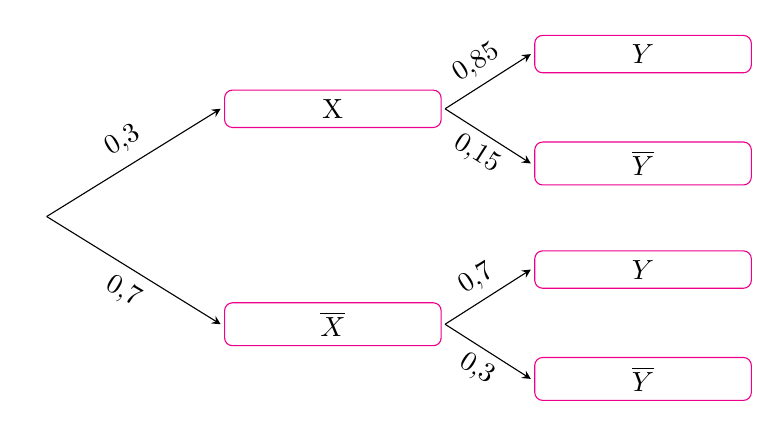
\begin{tikzpicture}
				\def\gocm{20}
				\def\gocn{10}
				\def\r{4}
				\tikzset{s/.style={outer sep=0.5 mm,draw=magenta,rectangle,minimum width=2.75cm,rounded corners=1mm}}
				\path(0,0)node(O){}++(\gocm:\r)node[s](A1){X}++(\gocn:\r)node[s](A2){$Y$};
				\path(A1)++({-\gocn}:\r)node[s](a2){$\overline{Y}$};
				\path(O)++(-\gocm:\r)node[s](B1){$\overline{X}$}++(\gocn:\r)node[s](B2){$Y$};
				\path(B1)++({-\gocn}:\r)node[s](b2){$\overline{Y}$};
				\foreach \x/\y in {
					O/A1,A1/A2,
					O/B1,B1/B2,
					A1/a2,
					B1/b2}
				\draw[-stealth](\x.east)--(\y.west);
				\path(O)--(A1.west)node[pos=0.5,above,sloped]{$0{,}3$}(O)--(B1.west)node[pos=0.5,below,sloped]{$0{,}7$}(B1.east)--(B2.west)node[pos=0.5,above,sloped]{$0{,}7$}(A1.east)--(A2.west)node[pos=0.5,above,sloped]{$0{,}85$}
				(A1.east)--(a2.west)node[pos=0.5,below,sloped]{$0{,}15$}
				(B1.east)--(b2.west)node[pos=0.5,below,sloped]{$0{,}3$};
			\end{tikzpicture}
		\end{center}
		Khi đó $\mathrm{P}\left(C\right)=\mathrm{P}\left(XY\right)=0{,}3\cdot 0{,}85=0{,}255$; $\mathrm{P}\left(B\right)=\mathrm{P}\left(\overline{X}Y\right)=0{,}7\cdot 0{,}7=0{,}49$.
	}
\end{vd}
%%%=============================%%%

\begin{dang}{Ứng dụng}
	\begin{itemize}
		\item Vận dụng công thức xác suất có điều kiện để giải quyết một số bài toán có liên quan đến thực tiễn.
	\end{itemize}
\end{dang}

%%%=============VD_1=============%%%
\begin{vd}%[2D6N1-2]
	Một doanh nghiệp trước khi xuất khẩu áo sơ mi trong lô hàng $S$ phải qua hai lần kiểm tra chất lượng sản phẩm, nếu cả hai lần đều đạt thì chiếc áo trong lô hàng đó mới đủ tiêu chuẩn xuất khẩu. Biết rằng bình quân $98\%$ sản phẩm làm ra qua được lần kiểm tra thứ nhất và $95\%$ sản phẩm qua được lần kiểm tra thứ nhất sẽ tiếp tục qua được lần kiểm tra thứ hai. Chọn ra ngẫu nhiên một chiếc áo sơ mi trong lô hàng $S$. Tính xác suất để một chiếc áo sơ mi đủ tiêu chuẩn xuất khẩu.
	\loigiai{
		Xét các biến cố:\\
		$A$: “Chiếc áo sơ mi qua được lần kiểm tra thứ nhất”;\\
		$B$: “Chiếc áo sơ mi qua được lần kiểm tra thứ hai”;\\
		$C$: “Chiếc áo sơ mi đủ tiêu chuẩn xuất khẩu”.\\
		Khi đó, xác suất để chiếc áo sơ mi qua được lần kiểm tra thứ hai, biết rằng đã qua được lần kiểm tra thứ nhất, là xác suất có điều kiện $\mathrm{P}\left(B\mid A\right)$ và $\mathrm{P}\left(C\right)=\mathrm{P}\left(B\cap A\right)$.\\
		Ta có $\mathrm{P}\left(B\mid A\right)=0{,}95$; $\mathrm{P}\left(A\right)=0{,}98$.\\
		Suy ra $\mathrm{P}\left(C\right)=\mathrm{P}\left(B\cap A\right)=\mathrm{P}\left(A\right)\cdot \mathrm{P}\left(B\mid A\right)=0{,}98\cdot0{,}95=0{,}931$.
		\\
		Vậy xác suất để một chiếc áo sơ mi đủ tiêu chuẩn xuất khẩu là $0{,}931$.
	}
\end{vd}
%%%=============================%%%

%%%=============VD_2=============%%%
\begin{vd}%[2D6H1-2]
	Một lô sản phẩm có $25$ sản phẩm, trong đó có $8$ sản phẩm chất lượng thấp. Lấy liên tiếp $2$ sản phẩm trong lô sản phẩm trên, trong đó sản phẩm lấy ra ở lần thứ nhất không được bỏ lại vào lô sản phẩm. Tính xác suất để cả hai sản phẩm được lấy	ra đều có chất lượng thấp.
	\loigiai{
		Xét các biến cố:\\
		$A$: “Lần thứ nhất lấy ra sản phẩm chất lượng thấp”;\\
		$B$: “Lần thứ hai lấy ra sản phẩm chất lượng thấp”;\\
		$C$: “Cả hai lần đều lấy ra sản phẩm chất lượng thấp”.\\
		Khi đó, xác suất để lần thứ hai lấy ra sản phẩm chất lượng thấp, biết lần thứ nhất lấy ra sản phẩm chất lượng thấp, là xác suất có điều kiện $\mathrm{P}\left(B\mid A\right)$ và $\mathrm{P}\left(C\right)=\mathrm{P}\left(B\cap A\right)$.\\
		Ta có $\mathrm{P}\left(A\right)=\dfrac{8}{25}$; $\mathrm{P}\left(B\mid A\right)=\dfrac{7}{24}$.\\
		Suy ra $\mathrm{P}\left(C\right)=\mathrm{P}\left(B\cap A\right)=\mathrm{P}\left(A\right)\cdot \mathrm{P}\left(B\mid A\right)=\dfrac{8}{25}\cdot\dfrac{7}{24}=\dfrac{7}{75}$.\\
		Vậy xác suất để cả hai sản phẩm được lấy ra đều có chất lượng thấp là $\dfrac{7}{75}$.
	}
\end{vd}
%%%=============================%%%

%%%=============VD_3=============%%%
\begin{vd}%[2D5V1-2]
	Kết quả khảo sát những bệnh nhân bị tai nạn xe máy về mối liên hệ giữa việc đội mũ bảo hiểm và khả năng bị chấn thương vùng đầu cho thấy:\\
	- Tỉ lệ bệnh nhân bị chấn thương vùng đầu khi gặp tai nạn là $80 \%$;\\
	- Tỉ lệ bệnh nhân đội mũ bảo hiểm đúng cách khi gặp tai nạn là $90 \%$;\\
	- Tỉ lệ bệnh nhân đội mũ bảo hiểm đúng cách bị chấn thương vùng đầu là $18 \%$.\\
	Hỏi theo kết quả điều tra trên, việc đội mũ bảo hiểm đúng cách sẽ làm giảm khả năng bị chấn thương vùng đầu bao nhiêu lần?
	\loigiai{
		Gọi $A$ là biến cố: \lq\lq Bệnh nhân bị chấn thương vùng đầu khi gặp tai nạn\rq\rq\, và B là biến cố: \lq\lq Bệnh nhân đội mũ bảo hiểm đúng cách khi gặp tai nạn\rq\rq.\\
		Theo đề bài ta có $\mathrm{P}\left(A\right)=0{,}8$;	 $\mathrm{P}\left(B\right)=0{,}9$; $\mathrm{P}\left(B\mid A\right)=0{,}18$.\\
		Suy ra $\mathrm{P}\left(B\mid A\right)=\dfrac{\mathrm{P}\left(AB\right)}{\mathrm{P}\left(A\right)}\Rightarrow \mathrm{P}\left(AB\right)=\mathrm{P}\left(A\right)\cdot \mathrm{P}\left(B\mid A\right)=0{,}8\cdot 0{,}18=0{,}144$.\\
		Vì $A\overline{B}$ và $AB$ là hai biến cố xung khắc nên $A\overline{B}\cup AB=A$.\\
		Suy ra $\mathrm{P}\left(\overline{B}A\right)=\mathrm{P}\left(A\right)-\mathrm{P}\left(AB\right)=0{,}8-0{,}144=0{,}656$.\\
		Ta có $\mathrm{P}\left(\overline{B}\mid A\right)=\dfrac{\mathrm{P}\left(\overline{B}A\right)}{\mathrm{P}\left(A\right)}=\dfrac{0{,}656}{0{,}8}=0{,}82$.
		Khi đó $\dfrac{\mathrm{P}\left(\overline{B}|A\right)}{\mathrm{P}\left(B\mid A\right)}=\dfrac{0{,}82}{0{,18}}\approx 4{,}6$.\\
		Như vậy việc đội mũ bảo hiểm đúng cách sẽ làm giảm khả năng chấn thương vùng đầu xuống $4{,}6$ lần.
	}
\end{vd}
%%%=============================%%%
\subsection{BÀI TẬP RÈN LUYỆN}
\ind{PHẦN I.} \inden{Câu trắc nghiệm nhiều phương án lựa chọn. Mỗi câu hỏi học sinh chỉ chọn một phương án.}\\

\setcounter{ex}{0}
\Opensolutionfile{ans}[ans/2T1-Bai1-TN]%--Đặt tên 2T1-Bai1-Dang1-TN
%%%=============EX_1=============%%%
\begin{ex}[Trích đề thi số 18 - Bộ 30 đề thi thử MAPSTUDY - Năm học: 2024-2025]%[2D6N1-1]%[Dự án đề cương 3 khối NH24-25-Dot 1-Khắc Thiên]
	Cho các biến cố $A$ và $B$ thỏa mãn $\mathrm{P}\left(A\right)>0$, $\mathrm{P}\left(B\right)>0$. Khẳng định nào đúng?
	\choice
	{$\mathrm{P}\left(A \mid B\right)= \dfrac{\mathrm{P}\left(AB\right)}{\mathrm{P}\left(A\right)}$}
	{\True $\mathrm{P}\left(A \mid B\right)= \dfrac{\mathrm{P}\left(AB\right)}{\mathrm{P}\left(B\right)}$}
	{$\mathrm{P}\left(A \mid B\right)= \dfrac{\mathrm{P}\left(A\right)}{\mathrm{P}\left(AB\right)}$}
	{$\mathrm{P}\left(A \mid B\right)= \dfrac{\mathrm{P}\left(B\right)}{\mathrm{P}\left(AB\right)}$}
	\loigiai{
		Công thức xác suất có điều kiện $\mathrm{P}\left(A \mid B\right)= \dfrac{\mathrm{P}\left(AB\right)}{\mathrm{P}\left(B\right)}$.
	}
\end{ex}
%%%=============================%%%

%%%=============EX_2=============%%%
\begin{ex}[Trích đề thi HKII - Sở GD\&ĐT Kiên Giang - Năm học: 2024-2025]%[2D6N1-1]%[Dự án đề cương 3 khối NH24-25-Dot 1-Khắc Thiên]
	Cho $A$, $B$ là hai biến cố bất kì và $\mathrm{P}\left(B\right)>0$. Kí hiệu $A\cap B=AB$, công thức tính xác suất có điều kiện nào sau đây đúng?
	\choice
	{$\mathrm{P}\left(A\mid B\right)=\dfrac{\mathrm{P}\left(AB\right)}{\mathrm{P}\left(A\right)}$}
	{$\mathrm{P}\left(AB\right)=\dfrac{\mathrm{P}\left(A\mid B\right)}{\mathrm{P}\left(B\right)}$}
	{$\mathrm{P}\left(A\mid B\right)=\mathrm{P}\left(AB\right)\cdot \mathrm{P}\left(B\right)$}
	{\True $\mathrm{P}\left(A\mid B\right) =\dfrac{\mathrm{P}\left(AB\right)}{\mathrm{P}\left(B\right)}$}
	\loigiai{Công thức đúng là $\mathrm{P}\left(A\mid B\right)=\dfrac{\mathrm{P}\left(AB\right)}{\mathrm{P}\left(B\right)}$.}
\end{ex}
%%%=============================%%%

%%%=============EX_3=============%%%
\begin{ex}[Trích đề thi HKII - Trường THPT Marie Curie - TP. HCM - Năm học: 2024-2025]%[2D6N1-1]%[Dự án đề cương 3 khối NH24-25-Dot 1-Khắc Thiên]
	Cho $A$, $B$ là các biến cố của một phép thử $T$. Biết rằng $\mathrm{P}\left(B\right)>0$, xác suất của biến cố $A$ với điều kiện biến cố $B$ đã xảy ra được tính theo công thức nào sau đây?
	\choice
	{$\mathrm{P}\left(A \mid B\right)=\dfrac{\mathrm{P}\left(AB\right)}{\mathrm{P}\left(A\right) \cdot \mathrm{P}\left(B\right)}$}
	{\True $\mathrm{P}\left(A \mid B\right)=\dfrac{\mathrm{P}\left(AB\right)}{\mathrm{P}\left(B\right)}$}
	{$\mathrm{P}\left(A \mid B\right)=\dfrac{\mathrm{P}\left(A\right)}{\mathrm{P}\left(B\right)}$}
	{$\mathrm{P}\left(A \mid B\right) =\dfrac{\mathrm{P}\left(BA\right)}{\mathrm{P}\left(A\right)}$}
	\loigiai{
		Áp dụng lý thuyết ta có $\mathrm{P}\left(A \mid B\right)=\dfrac{\mathrm{P}\left(AB\right)}{\mathrm{P}\left(B\right)}$.}
\end{ex}
%%%=============================%%%

%%%=============EX_4=============%%%
\begin{ex}[Trích đề thi HKII - THPT Ngô Quyền - TP. HCM - Năm học: 2024 - 2025]%[2D6N1-1]%[Dự án đề cương 3 khối NH24-25-Dot 1-Khắc Thiên]
	Cho hai biến cố $A$ và $B$ với $\mathrm{P}\left(B\right)>0$ thì xác suất của biến cố $A$ với điều kiện biến cố $B$ đã xảy ra là
	\choice
	{\True $\mathrm{P}\left(A\mid B\right)=\dfrac{\mathrm{P}\left(AB\right)}{\mathrm{P}\left(B\right)}$}
	{$\mathrm{P}\left(A\mid B\right)=\dfrac{\mathrm{P}\left(A\right)}{\mathrm{P}\left(B\right)}$}
	{$\mathrm{P}\left(B\mid A\right)=\dfrac{\mathrm{P}\left(AB\right)}{\mathrm{P}\left(A\right)}$}
	{$\mathrm{P}\left(A\mid B\right)=\mathrm{P}\left(A\right)\mathrm{P}\left(B\right)$}
	\loigiai{Theo công thức xác suất có điều kiện, ta có $\mathrm{P}\left(A\mid B\right)=\dfrac{\mathrm{P}\left(AB\right)}{\mathrm{P}\left(B\right)}$.
	}
\end{ex}
%%%=============================%%%

%%%=============EX_5=============%%%
\begin{ex}[Trích đề thi thử sở GD\&ĐT Thừa Thiên Huế - Năm học: 2024-2025]%[2D6N1-2]%[Dự án đề cương 3 khối NH24-25-Dot 1-Khắc Thiên]
	Cho $A$ và $B$ là hai biến cố độc lập thoả mãn $\mathrm{P}\left(A\right)=0{,}5$ và $\mathrm{P}\left(B\right)= 0{,}3$. Khi đó $\mathrm{P}\left(A\cap B\right)$ bằng
	\choice
	{$0{,}8$}
	{$0{,}2$}
	{$0{,}6$}
	{\True $0{,}15$}
	\loigiai{
		$\mathrm{P}\left(A \cap B\right)=\mathrm{P}\left( A\right)\cdot\mathrm{P}\left(B\right)=0{,}5\cdot 0{,}3 = 0{,}15$.
	}
\end{ex}
%%%=============================%%%

%%%=============EX_6=============%%%
\begin{ex}[Trích đề thi HKII - Trường THPT Marie Curie - TP.HCM - Năm học: 2024-2025]%[2D6N1-2]%[Dự án đề cương 3 khối NH24-25-Dot 1-Khắc Thiên]
	Cho hai biến cố $A$ và $B$ có $\mathrm{P}\left(A\right)=0{,}8$; $\mathrm{P}\left(B\right)=0{,}5$ và $\mathrm{P}\left(AB\right)=0{,}2$. Xác suất của biến cố $A$ với điều kiện $B$ là
	\choice
	{$0{,}625$}
	{$0{,}5$}
	{$0{,}25$}
	{\True $0{,}4$}
	\loigiai{
		Ta có $\mathrm{P}\left(A \mid B\right)=\dfrac{\mathrm{P}\left(AB\right)}{\mathrm{P}\left(B\right)}=\dfrac{0{,}2}{0{,}5}=0{,}4$.
	}
\end{ex}
%%%=============================%%%

%%%=============EX_7=============%%%
\begin{ex}[Trích đề thi HKII - Trường THPT Ngô Gia Tự - Phú Yên - Năm học: 2024-2025]%[2D6N1-2]%[Dự án đề cương 3 khối NH24-25-Dot 1-Khắc Thiên]
	Cho hai biến cố $A$, $B$ có $\mathrm{P}\left(A\right)=0{,}6$; $\mathrm{P}\left(B\right)=0{,}7$; $\mathrm{P}\left(AB\right)=0{,}4$. Xác suất $\mathrm{P}\left(A\mid B\right)$ bằng
	\choice
	{$\dfrac{6}{7}$}
	{\True $\dfrac{4}{7}$}
	{$0{,}28$}
	{$\dfrac{2}{3}$}
	\loigiai{$\mathrm{P}\left(A\mid B\right)=\dfrac{\mathrm{P}\left(AB\right)}{\mathrm{P}\left(B\right)}=\dfrac{0{,}4}{0{,}7}=\dfrac{4}{7}$.}
\end{ex}
%%%=============================%%%

%%%=============EX_8=============%%%
\begin{ex}[Trích đề thi HKII - Trường THPT Ngô Gia Tự - Phú Yên - Năm học: 2024-2025]%[2D6N1-2]%[Dự án đề cương 3 khối NH24-25-Dot 1-Khắc Thiên]
	Cho $A$ và $B$ hai biến cố độc lập. Khẳng định nào dưới đây là \textbf{sai}?
	\choice
	{\True $\mathrm{P}\left(B\mid A\right)=\mathrm{P}\left(A\right)$}
	{$\mathrm{P}\left(A\mid B\right)=\mathrm{P}\left(A\right)$}
	{$\mathrm{P}\left(\overline{A}\mid B\right)=\mathrm{P}\left(\overline{A}\right)$}
	{$\mathrm{P}\left(A\mid \overline{B}\right)=\mathrm{P}\left(A\right)$}
	\loigiai{
		Với $A$ và $B$ hai biến cố độc lập thì $\mathrm{P}\left(B\mid A\right)=\mathrm{P}\left(B\right)$.\\
		Do đó khẳng định $\mathrm{P}\left(B\mid A\right)=\mathrm{P}\left(A\right)$ là sai.
	}
\end{ex}
%%%=============================%%%

%%%=============EX_9=============%%%
\begin{ex}[Trích đề thi HKII - Trường THPT Ngô Gia Tự - Phú Yên - Năm học: 2024-2025]%[2D6N1-2]%[Dự án đề cương 3 khối NH24-25-Dot 1-Khắc Thiên]
	Cho hai biến cố $A$ và $B$ với $\mathrm{P}(A)>0$. Xác suất của biến cố $B$ với điều kiện biến cố $A$ đã xảy ra là
	\choice
	{$\mathrm{P}\left(B\mid A\right)=\dfrac{\mathrm{P}\left(A\right)}{\mathrm{P}\left(B\right)}$}
	{$\mathrm{P}\left(B\mid A\right)=\mathrm{P}\left(A\right)\cdot \mathrm{P}\left(B\right)$}
	{\True $\mathrm{P}\left(B\mid A\right)=\dfrac{\mathrm{P}\left(AB\right)}{\mathrm{P}\left(A\right)}$}
	{$\mathrm{P}\left(B\mid A\right)=\dfrac{\mathrm{P}\left(AB\right) }{\mathrm{P}\left(B\right)}$}
	\loigiai{Theo công thức xác suất có điều kiện ta có $\mathrm{P}\left(B\mid A\right)=\dfrac{\mathrm{P}\left(AB\right)}{\mathrm{P}\left(A\right)}$.
	}
\end{ex}
%%%=============================%%%

%%%=============EX_10=============%%%
\begin{ex}[Trích đề thi HKII - Trường THPT Thuận Thành số 1 - Bắc Ninh - Năm học: 2024-2025]%[2D6N1-2]%[Dự án đề cương 3 khối NH24-25-Dot 1-Khắc Thiên]
	Lớp $12A$ có $30$ học sinh, trong đó có $17$ bạn nữ, còn lại là nam. Có $3$ bạn tên Hiền, trong đó có $1$ bạn nữ và $2$ bạn nam. Thầy giáo gọi ngẫu nhiên $1$ bạn lên bảng. Xác suất để bạn đó có tên Hiền, với điều kiện bạn đó là nữ, là
	\choice
	{$\dfrac{1}{17}$}
	{$\dfrac{3}{17}$}
	{$\dfrac{17}{30}$}
	{\True $\dfrac{13}{30}$}
	\loigiai{
		Gọi biến cố
		\begin{itemize}
			\item $A$: \lq\lq Học sinh được gọi lên bảng tên là Hiền\rq\rq.
			\item $B$: \lq\lq Học sinh được chọn mang giới tính nữ\rq\rq.
		\end{itemize}
		Xác suất để thầy giáo gọi bạn đó lên bảng tên Hiền với điều kiện bạn đó là nữ là $\mathrm{P}\left(A \mid B\right)$.\\
		Ta có $n\left(B\right)=17$, $n\left(A \cap B\right)=1$.\\
		Do đó
		$\mathrm{P}\left(A \mid B\right)=\dfrac{\mathrm{P}\left(A \cap B\right)}{\mathrm{P}\left(B\right)}=\dfrac{n\left(A \cap B\right)}{n\left(B\right)}=\dfrac{1}{17}$.
	}
\end{ex}
%%%=============================%%%

%%%=============EX_11=============%%%
\begin{ex}[Trích đề thi số 7 - Bộ 30 đề thi thử MAPSTUDY - Năm học: 2024-2025]%[2D6H1-2]%[Dự án đề cương 3 khối NH24-25-Dot 1-Khắc Thiên]
	Cho $A$ và $B$ là hai biến cố trong cùng $1$ phép thử và $\mathrm{P}\left(B\right)=0{,}5$; $\mathrm{P}\left(A \mid B\right)=0{,}8$. Khi đó $\mathrm{P}\left(AB\right)$ bằng bao nhiêu?
	\choice
	{$0{,}25$}
	{$0{,}6$}
	{$0{,}8$}
	{\True $0{,}4$}
	\loigiai{
		Ta có $\mathrm{P}\left(AB\right)=\mathrm{P}\left(A \mid B\right) \cdot \mathrm{P}\left(B\right) =0{,}8 \cdot 0{,}5=0{,}4$.
	}
\end{ex}
%%%=============================%%%

%%%=============EX_12=============%%%
\begin{ex}[Trích đề số 16 - Bộ 30 đề thi thử MAPSTUDY - Năm học: 2024-2025]%[2D6H1-2]%[Dự án đề cương 3 khối NH24-25-Dot 1-Khắc Thiên]
	Cho $\mathrm{P}\left(A\right)=\dfrac{3}{10}$; $\mathrm{P}\left(B\right)=\dfrac{2}{5}$ và $\mathrm{P}\left(A \cup B\right)=\dfrac{3}{5}$. Tính $\mathrm{P}\left(B \mid A\right)$.
	\choice
	{$\dfrac{7}{12}$}
	{$\dfrac{11}{12}$}
	{\True $\dfrac{1}{3}$}
	{$\dfrac{5}{12}$}
	\loigiai{
		Ta có $\mathrm{P}\left(A \cup B\right) =\mathrm{P}\left(A\right)+\mathrm{P}\left(B\right)-\mathrm{P}\left(AB\right) \Leftrightarrow \mathrm{P}\left(AB\right)=\mathrm{P}\left(A\right)+\mathrm{P}\left(B\right)-\mathrm{P}\left(A\cup B\right) =\dfrac{3}{10}+\dfrac{2}{5}-\dfrac{3}{5}=\dfrac{1}{10}$.\\
		Do đó $\mathrm{P}\left(B\mid A\right) =\dfrac{\mathrm{P}\left( AB\right) }{\mathrm{P}\left(A\right)}=\dfrac{\dfrac{1}{10}}{\dfrac{3}{10}}=\dfrac{1}{3}$.
	}
\end{ex}
%%%=============================%%%

%%%=============EX_13=============%%%
\begin{ex}[Trích đề thi thử thực chiến số 7 - Bộ đề thi thử thầy Đỗ Văn Đức - Năm học: 2024 - 2025]%[2D6H1-2]
	Cho $A$ và $B$ là hai biến cố trong cùng $1$ phép thử và $\mathrm{P}(B)=0{,}5$; $\mathrm{P}(A \mid B)=0{,}8$. Khi đó $\mathrm{P}(AB)$ bằng bao nhiêu?
	\choice
	{$0{,}25$}
	{$0{,}6$}
	{$0{,}8$}
	{\True $0{,}4$}
	\loigiai{
		Ta có \[\mathrm{P}(AB)=\mathrm{P}(A \mid B) \cdot \mathrm{P}(B)  =0{,}8 \cdot 0{,}5=0{,}4\]
	}
\end{ex}
%%%=============================%%%

%%%=============EX_14=============%%%
\begin{ex}[Trích đề thi thử số 17 - Bộ đề thi thử của thầy Phan Nhật Linh - Năm học: 2024-2025]%[2D6H1-2]%[Dự án đề cương 3 khối NH24-25-Dot 1-Khắc Thiên]
	Để được chọn vào đội tuyển học sinh giỏi môn Toán cấp thành phố, mỗi thí sinh phải vượt qua hai vòng thi. Bạn An tham dự cuộc tuyển chọn này. Xác suất để An qua được vòng thứ nhất là $0{,}8$. Nếu qua được vòng thứ nhất thì xác suất để An qua được vòng thứ hai là $0{,}7$. Xác suất để bạn An được chọn vào đội tuyển này là
	\choice
	{$0{,}06$}
	{$0{,}24$}
	{\True $0{,}56$}
	{$0{,}875$}
	\loigiai{
		Gọi $A$ là biến cố: \lq\lq An qua được vòng thứ nhất\rq\rq~và $B$ là biến cố: \lq\lq An qua được vòng thứ hai\rq\rq.\\
		Khi đó biến cố: \lq\lq An được chọn vào đội tuyển\rq\rq~là $AB$.\\
		Do đó $\mathrm{P}\left(AB\right)= \mathrm{P}\left(A\right)\cdot \mathrm{P}\left(B\mid A\right)= 0{,}8\cdot 0{,}7=0{,}56$.
	}
\end{ex}
%%%=============================%%%

%%%=============EX_15=============%%%
\begin{ex}[Trích đề thi HKII - Trường THPT Marie Curie - TP.HCM - Năm học: 2024-2025]%[2D6H1-2]%[Dự án đề cương 3 khối NH24-25-Dot 1-Khắc Thiên]
	Một cuộc thi đánh giá năng lực có hai vòng. Thí sinh đỗ nếu vượt qua được cả hai vòng. Bình tham dự kì thi này. Xác suất để Bình qua được vòng $1$ là $0{,}9$. Nếu qua được vòng $1$ thì xác suất để Bình qua được vòng $2$ là $0{,}8$. Xác suất để Bình đỗ được kì thi này là
	\choice
	{$1$}
	{\True $0{,}72$}
	{$0{,}65$}
	{$0{,}82$}
	\loigiai{
		Gọi $A\colon$ \lq\lq Bình qua vòng $1$\rq\rq;
		$B\colon$ \lq\lq Bình qua vòng $2$\rq\rq .\\
		Ta có $\mathrm{P}\left(A\right)=0{,}9$; $\mathrm{P}\left(B\mid A\right)=0{,}8$.\\
		Xác suất để Bình đỗ kì thi là xác suất để Bình qua cả hai vòng, tức là\\
		$\mathrm{P}\left(A\cap B\right)=\mathrm{P}\left( A\right)\cdot \mathrm{P}\left(B \mid A\right)
		\Rightarrow
		\mathrm{P}\left(A\cap B\right)= 0{,}9 \cdot 0{,}8 = 0{,}72$.\\
		Vậy xác suất để Bình đỗ kì thi là $0{,}72$.
	}
\end{ex}
%%%=============================%%%

%%%=============EX_16=============%%%
\begin{ex}[Trích đề thi HKII - Trường THPT Nguyễn Gia Thiều - Hà Nội - Năm học: 2024-2025]%[2D6H1-2]%[Dự án đề cương 3 khối NH24-25-Dot 1-Khắc Thiên]
	Cho hai biến cố $A$, $B$ sao cho $\mathrm{P}\left(A\right)=0{,}6$; $\mathrm{P}\left(B\right)=0{,}5$; $\mathrm{P}\left(A\mid B\right)=0{,}2$. Khi đó $\mathrm{P}\left(B\mid A\right)$ bằng
	\choice
	{$\dfrac{6}{25}$}
	{$\dfrac{3}{25}$}
	{\True $\dfrac{1}{6}$}
	{$\dfrac{1}{3}$}
	\loigiai{
		Ta có công thức xác suất có điều kiện $\mathrm{P}\left(A\mid B\right)= \dfrac{\mathrm{P}\left(A\cap B\right)}{\mathrm{P}\left(B\right)}$.\\
		Từ đó suy ra $\mathrm{P}\left(A \cap B\right)= \mathrm{P}\left(A\mid B\right)\cdot \mathrm{P}\left(B\right)= 0{,}2 \cdot 0{,}5 = 0{,}1$.\\
		Ta cần tính $\mathrm{P}\left(B\mid A\right)$. Theo công thức $\mathrm{P}\left(B\mid A\right)= \dfrac{\mathrm{P}\left(B\cap A\right)}{\mathrm{P}\left(A\right)}$.\\
		Vì $A \cap B=B \cap A$, nên $\mathrm{P}\left(A \cap B\right)=\mathrm{P}\left(B \cap A\right)= 0{,}1$.\\
		Vậy $\mathrm{P}\left(B\mid A\right)=
		\dfrac{0{,}1}{0{,}6}=\dfrac{1}{6}$.
	}
\end{ex}
%%%=============================%%%

%%%=============EX_17=============%%%
\begin{ex}[Trích đề thi HKII - Trường THPT Nguyễn Gia Thiều - Hà Nội - Năm học: 2024-2025]%[2D6H1-2]%[Dự án đề cương 3 khối NH24-25-Dot 1-Khắc Thiên]
	Cho hai biến cố $A$, $B$ với $\mathrm{P}\left( B\right)=0{,}6$; $\mathrm{P}\left(A\mid B\right)=0{,}5$. Khi đó $\mathrm{P}\left(AB\right)$ bằng
	\choice
	{\True $\dfrac{3}{10}$}
	{$\dfrac{5}{6}$}
	{$\dfrac{1}{2}$}
	{$\dfrac{3}{5}$}
	\loigiai{
		Theo công thức xác suất có điều kiện ta có $\mathrm{P}\left(A\mid B\right)= \dfrac{\mathrm{P}\left(AB\right)}{\mathrm{P}\left(B\right)}$.\\
		Suy ra $\mathrm{P}\left(AB\right)= \mathrm{P}\left(A\mid B\right)\cdot \mathrm{P}\left(B\right)=0{,}5 \cdot 0{,}6=0{,}3=\dfrac{3}{10}$.\\
		Vậy $\mathrm{P}\left(AB\right)=\dfrac{3}{10}$.
	}
\end{ex}
%%%=============================%%%

%%%=============EX_18=============%%%
\begin{ex}[Trích đề thi HKII - Trường THPT Nguyễn Gia Thiều - Hà Nội - Năm học: 2024-2025]%[2D6H1-2]%[Dự án đề cương 3 khối NH24-25-Dot 1-Khắc Thiên]
	Cho bảng dữ liệu sau về kết quả xét nghiệm một loại bệnh
	\begin{center}
		\begin{tabular}{|l|c|c|}
			\hline
			& Dương tính & Âm tính \\
			\hline
			Bệnh & $120$ & $30$ \\
			\hline
			Không bệnh & $40$ & $970$ \\
			\hline
		\end{tabular}
	\end{center}
	Nếu một người có kết quả xét nghiệm dương tính, xác suất người đó thực sự mắc bệnh là
	\choice
	{$3\%$}
	{$11\%$}
	{\True $75\%$}
	{$90\%$}
	\loigiai{
		Gọi biến cố $A$ \lq \lq người được xét nghiệm thực sự mắc bệnh\rq \rq.\\
		Gọi biến cố $B$ \lq \lq người được xét nghiệm có kết quả dương tính\rq \rq .\\
		Chúng ta cần tính xác suất có điều kiện $\mathrm{P}\left(A\mid B\right)$.\\
		Dựa vào bảng dữ liệu
		\begin{itemize}
			\item Số người mắc bệnh và có kết quả dương tính (biến cố $A \cap B$) là $120$ người.
			\item Số người không mắc bệnh và có kết quả dương tính là $40$ người.
		\end{itemize}
		Tổng số người có kết quả xét nghiệm dương tính (biến cố $B$) là $120 + 40 = 160$ người.\\
		Xác suất để một người thực sự mắc bệnh, biết rằng người đó có kết quả xét nghiệm dương tính là
		$$ \mathrm{P}\left(A\mid B\right)=\dfrac{n(A\cap B)}{n(B)}=\dfrac{120}{160}=\dfrac{12}{16} = \dfrac{3}{4}=0{,}75=75\%.$$
	}
\end{ex}
%%%=============================%%%

%%%=============EX_19=============%%%
\begin{ex}[Trích đề thi HKII - Trường THPT Quế Sơn - Quảng Nam - Năm học: 2024-2025]%[2D6H1-2]%[Dự án đề cương 3 khối NH24-25-Dot 1-Khắc Thiên]
	Gieo $2$ con xúc xắc cân đối đồng chất. Tính xác suất $\mathrm{P}$ để có ít nhất $1$ con xúc xắc xuất hiện mặt $3$ chấm nếu biết rằng tổng số chấm xuất hiện trên $2$ con xúc xắc bằng $8$.
	\choice
	{$\mathrm{P}=\dfrac{5}{12}$}
	{$\mathrm{P}=\dfrac{5}{11}$}
	{$\mathrm{P}=\dfrac{2}{11}$}
	{\True $\mathrm{P}=\dfrac{2}{5}$}
	\loigiai{
		Vì tổng số chấm xuất hiện trên hai con xúc xắc bằng $8$ nên có các kết quả
		$(2;6)$; $(6;2)$; $(3;5)$; $(5;3)$ và $(4;4)$. \\
		Số kết quả có thể xảy ra là $5$. \\
		Các kết quả để ít nhất $1$ con xúc xắc xuất hiện mặt $3$ chấm là $(3;5)$ và $(5;3)$. \\
		Số kết quả thuận lợi là $2$. \\
		Vậy $\mathrm{P}=\dfrac{2}{5}$.
	}
\end{ex}
%%%=============================%%%

%%%=============EX_20=============%%%
\begin{ex}[Trích đề thi HKII - Trường THPT Lê Quý Đôn - Quảng Ngãi - Năm học: 2024-2025]%[2D6H1-2]%[Dự án đề cương 3 khối NH24-25-Dot 1-Khắc Thiên]
	Cho $\mathrm{P}\left(B\right)=0{,}4$ và $\mathrm{P}\left(A\mid B\right)=0{,}8$. Tính $\mathrm{P}\left(AB\right)$.
	\choice
	{$\mathrm{P}\left(AB\right)=1$}
	{$\mathrm{P}\left(AB\right)=0{,}8$}
	{$\mathrm{P}\left(AB\right)=0{,}4$}
	{\True $\mathrm{P}\left(AB\right)=0{,}32$}
	\loigiai{Ta có $\mathrm{P}\left(AB\right)= \mathrm{P}\left(B\right)\cdot \mathrm{P}\left(A\mid B\right)= 0{,}4\cdot 0{,}8 = 0{,}32$.
	}
\end{ex}
%%%=============================%%%
\Closesolutionfile{ans}
\ind{PHẦN II.} \inden{Câu trắc nghiệm đúng sai. Trong mỗi ý a), b), c), d) ở mỗi câu, học sinh chọn đúng hoặc sai.}\\
\setcounter{ex}{0}
\Opensolutionfile{ans}[ans/2T6-Bai1-DS]
%%%=============EX_1=============%%%
\begin{ex}[Trích đề thi thi thử số 7 - Sở GD\&ĐT Huế - Năm học: 2024 - 2025]%[2D6H1-2]
	Khi kiểm tra sức khoẻ tổng quát của bệnh nhân ở một bệnh viện, người ta được kết quả như sau
	\begin{itemize}
		\item Có $40\%$ bệnh nhân bị đau dạ dày
		\item Có $30\%$ bệnh nhân thường xuyên bị stress
		\item Trong số các bệnh nhân bị stress có $80\%$ bệnh nhân bị đau dạ dày
	\end{itemize}
	Chọn ngẫu nhiên $1$ bệnh nhân.
	\choiceTF
	{\True Xác suất chọn được bệnh nhân thường xuyên bị stress là $0{,}3$}
	{\True Xác suất chọn được bệnh nhân bị đau dạ dày, biết bệnh nhân đó thường xuyên bị stress là $0{,}8$}
	{\True Xác suất chọn được bệnh nhân vừa thường xuyên bị stress vừa bị đau dạ dày là $0{,}24$}
	{\True Xác suất chọn được bệnh nhân thường xuyên bị stress, biết bệnh nhân đó bị đau dạ dày là $0{,}6$}
	\loigiai
	{\begin{itemchoice}
			\itemch
			Xét biến cố: $A$: \lq\lq Chọn được bệnh nhân thường xuyên bị stress\rq\rq. Ta có $\mathrm{P}(A) = 0{,}3$.
			\itemch
			Biến cố $B$: \lq\lq Chọn được bệnh nhân bị đau dạ dày\rq\rq, $\mathrm{P}(B) = 0{,}4$.\\
			Biến cố $B\mid A$: \lq\lq Bệnh nhân bị stress có bị đau dạ dày\rq\rq. Ta có $\mathrm{P}(B\mid A) = 0{,}8$.
			\itemch
			Xác suất chọn được bệnh nhân thường xuyên bị stress vừa bị đau dạ dày là
			\begin{eqnarray*}
				\mathrm{P}\left(A \cap B\right) = \mathrm{P}(A)\cdot \mathrm{P}(B\mid A)=0{,}3 \cdot 0{,}8 = 0{,}24.
			\end{eqnarray*}
			\itemch
			Xác suất chọn được bệnh nhân thường xuyên bị stress, biết bệnh nhân đó bị đau dạ dày là
			\begin{eqnarray*}
				\mathrm{P}\left(A\mid B\right) =\dfrac{\mathrm{P}\left(A\cap B\right)}{\mathrm{P}(B)}= \dfrac{0{,}24}{0{,}4} = 0{,}6.
			\end{eqnarray*}
		\end{itemchoice}
	}
\end{ex}
%%%=============================%%%

%%%=============EX_2=============%%%
\begin{ex}[Trích đề thi HKII - Trường THPT Ngô Gia Tự - Phú Yên - Năm học: 2024-2025]%[2D6H1-2]%[Dự án đề cương 3 khối NH24-25-Dot 1-Khắc Thiên]
	Một lớp học có $40$ học sinh gồm $28$ nữ và $12$ nam. Trong năm học $2023-2024$, có $7$ học sinh
	nữ đạt danh hiệu học sinh giỏi và $6$ học sinh nam đạt danh hiệu học sinh giỏi. Chọn ngẫu nhiên một
	học sinh của lớp đó. Gọi $A$ là biến cố \lq\lq Học sinh được chọn là nữ\rq\rq~và $B$ là biến cố \lq\lq Học sinh được chọn đạt danh hiệu học sinh giỏi\rq\rq.
	\choiceTF
	{\True Xác suất của biến cố $A$ là $0{,}7$}
	{Xác suất của biến cố $B$ là $0{,}3$}
	{$A$ và $B$ là hai biến cố độc lập}
	{Xác suất của biến cố $A$ với điều kiện biến cố $B$ đã xảy ra là $0{,}25$}
	\loigiai{
		\begin{itemchoice}
			\itemch
			$\mathrm{P}\left(A\right) =\dfrac{28}{28+12}=0{,}7$.
			\itemch
			Số học sinh giỏi là $7+6=13$ (học sinh).
			Suy ra $\mathrm{P}\left(B\right) =\dfrac{13}{40}=0{,}325$.
			\itemch
			Xác suất của biến cố $AB$ là
			$\mathrm{P}\left(AB\right)=\dfrac{7}{40}=0{,}175$.\\
			Ta có $\mathrm{P}\left(A\right)\cdot\mathrm{P}\left(B\right)=0{,}7\cdot 0{,}325=0{,}2275\neq \mathrm{P}\left(AB\right)$.\\
			Suy ra $A$ và $B$ không là hai biến cố độc lập
			\itemch Ta có $\mathrm{P}\left(A\mid B\right)=\dfrac{\mathrm{P}\left(AB\right)}{\mathrm{P}\left(B\right)}=\dfrac{0{,}175}{0{,}325}\approx 0{,}54$.
		\end{itemchoice}
	}
\end{ex}
%%%=============================%%%

%%%=============EX_3=============%%%
\begin{ex}[Trích đề thi HKII - Trường THPT Lê Quý Đôn - Quảng Ngãi - Năm học: 2024-2025]%[2D6H1-2]%[Dự án đề cương 3 khối NH24-25-Dot 1-Khắc Thiên]
	Để thử nghiệm tác dụng điều trị bệnh mất ngủ của hai loại thuốc $X$ và thuốc $Y$, người ta tiến hành thử nghiệm $5\,000$ bệnh nhân. Kết quả cho trong bảng thống kê $2\times 2$ sau
	\begin{center}
		\begin{tabular}{|c|c|c|}
			\hline
			\diagbox{Kết quả}{Dùng thuốc} & X & Y \\
			\hline
			Khỏi bệnh & $2\,000$ & $1\,500$\\
			\hline
			Không khỏi bệnh & $500$ & $1\,000$\\
			\hline
		\end{tabular}
	\end{center}
	Chọn ngẫu nhiên một bệnh nhân trong $5\,000$ bệnh nhân trên. Gọi $A$ là biến cố: \lq\lq Bệnh nhân khỏi bệnh\rq\rq; $B$ là biến cố: \lq\lq Bệnh nhân dùng thuốc X\rq\rq.
	\choiceTF
	{Số phần tử của biến cố $B$ là $n\left(B\right)=3\,500$}
	{\True Số phần tử của biến cố $A$ giao $B$ là $n\left(AB\right)=2\,000$}
	{\True Xác suất của biến cố $A$ với điều kiện $B$ là $\mathrm{P}\left(A\mid B\right)=\dfrac{4}{5}$}
	{\True Xác suất của biến cố $A$ là $\mathrm{P}\left(A\right)=\dfrac{7}{10}$}
	\loigiai{
		\begin{itemchoice}
			\itemch Theo bảng thống kê, số bệnh nhân dùng thuốc X là $2\,000 + 500 = 2\,500$.\\
			Do đó, số phần tử của biến cố $B$ là $n\left(B\right)=2\,500$.
			\itemch Theo bảng thống kê, số bệnh nhân khỏi bệnh và có dùng thuốc X là $2\,000$.\\
			Do đó, số phần tử của biến cố $A$ giao $B$ là $n\left(AB\right)= 2\,000$.
			\itemch Ta có $n\left(\Omega\right)= 5\,000$ nên
			\begin{itemize}
				\item $\mathrm{P}\left(B\right)= \dfrac{n\left(B\right)}{n\left(\Omega\right)}=\dfrac{2\,500}{5\,000}=\dfrac{1}{2}$.
				\item $\mathrm{P}\left(AB\right)= \dfrac{n\left(AB\right)}{n\left(\Omega\right)}=\dfrac{2\,000}{5\,000}=\dfrac{2}{5}$.
			\end{itemize}
			Xác suất của biến cố $A$ với điều kiện $B$ là $\mathrm{P}\left(A\mid B\right)= \dfrac{\mathrm{P}\left(AB\right)}{\mathrm{P}\left(B\right)}=\dfrac{\dfrac{2}{5}}{\dfrac{1}{2}}=\dfrac{4}{5}$.
			\itemch Theo bảng thống kê, số bệnh nhân khỏi bệnh là $2\,000 + 1\,500 = 3\,500$.\\
			Do đó, số phần tử của biến cố $A$ là $n\left(A\right)=3\,500$.\\
			Xác suất của biến cố $A$ là $\mathrm{P}\left(A\right)=\dfrac{n\left(B\right)}{n\left(\Omega\right)}=\dfrac{3\,500}{5\,000}=\dfrac{7}{10}$.
		\end{itemchoice}
	}
\end{ex}
%%%=============================%%%

%%%=============EX_4=============%%%
\begin{ex}[Trích đề thi thử thực chiến số 1 - Bộ đề thi thử thầy Đỗ Văn Đức - Năm học: 2024 - 2025]%[2D6V1-2]
	Trong một lễ hội học đường có trò chơi ném bowling, người chơi cầm bóng ném vào $10$ cái ki (hay còn gọi là pin) được xếp thành hình tam giác ở cuối đường băng (lane). Để dành chiến thắng, người chơi phải ném đổ hết các ki. Qua các năm trước người ta thống kê được chỉ có $10 \%$ người tham gia thành công làm đổ hết các ki. Xét $7$ bạn tham gia liên tiếp được chọn ngẫu nhiên. Gọi các biến cố \\
	$A$: \lq\lq Hai người cuối cùng thắng\rq\rq.\\
	$B$: \lq\lq Có đúng ba người thắng và họ đứng cạnh nhau\rq\rq.
	\choiceTF
	{$\mathrm{P}(A)=\mathrm{C}_7^2 \cdot 0{,}1^2$}
	{$\mathrm{P}(B)=0{,}005$}
	{$\mathrm{P}(B \mid A)=0{,}1$}
	{\True $\mathrm{P}(A \mid B)=0{,}2$}
	\loigiai{ Kí hiệu W là người chơi thắng cuộc; L là người chơi thua cuộc.
		\begin{itemchoice}
			\itemch
			Xác suất hai người chơi cuối cùng thắng cuộc là
			\[\mathrm{P}(A)= 0{,}1^2.\]
			\itemch
			Ta xét các trường hợp sau
			\begin{itemize}
				\item {\bf Trường hợp 1.} Ba người chơi đầu tiên thắng cuộc
				\begin{center}
					\begin{tabular}{ccccccc}
						W & W & W &L&L &L & L
					\end{tabular}
				\end{center}
				Xác suất trong trường hợp này là $P_1=0{,}1^3\cdot 0{,}9^4$.
				\item {\bf Trường hợp 2.} Ba người chơi thứ $2$, $3$, $4$ thắng cuộc
				\begin{center}
					\begin{tabular}{ccccccc}
						L & W & W &W&L &L & L
					\end{tabular}
				\end{center}
				Xác suất trong trường hợp này là $P_2=0{,}1^3\cdot 0{,}9^4$.
				\item {\bf Trường hợp 3.} Ba người chơi thứ $3$, $4$, $5$ thắng cuộc
				\begin{center}
					\begin{tabular}{ccccccc}
						L & L & W &W&W &L & L
					\end{tabular}
				\end{center}
				Xác suất trong trường hợp này là $P_3=0{,}1^3\cdot 0{,}9^4$.
				\item {\bf Trường hợp 4.} Ba người chơi thứ $4$, $5$, $6$ thắng cuộc
				\begin{center}
					\begin{tabular}{ccccccc}
						L & L & L &W&W &W & L
					\end{tabular}
				\end{center}
				Xác suất trong trường hợp này là $P_4=0{,}1^3\cdot 0{,}9^4$.
				\item {\bf Trường hợp 5.} Ba người chơi thứ $5$, $6$, $7$ thắng cuộc
				\begin{center}
					\begin{tabular}{ccccccc}
						L & L & L &L&W &W & W
					\end{tabular}
				\end{center}
				Xác suất trong trường hợp này là $P_5=0{,}1^3\cdot 0{,}9^4$.
			\end{itemize}
			Vây $\mathrm{P}(B)= 5\cdot 0{,}1^3\cdot 0{,}9^4\approx 0{,}00328$.
			\itemch
			Ta có $\mathrm{P}\left(B\mid A\right)=\dfrac{\mathrm{P}(AB)}{\mathrm{P}(A)}=\dfrac{P_5}{\mathrm{P}(A)}=\dfrac{0{,}1^3\cdot 0{,}9^4}{0{,}1^2}=0{,}06561$
			\itemch
			Ta có $\mathrm{P}(A \mid B)=\dfrac{\mathrm{P}(AB)}{\mathrm{P}(B)}=\dfrac{P_5}{\mathrm{P}(B)}=\dfrac{0{,}1^3\cdot 0{,}9^4}{5\cdot 0{,}1^3\cdot 0{,}9^4}=\dfrac{1}{5}=0{,}2$.
		\end{itemchoice}
	}
\end{ex}
%%%=============================%%%

%%%=============EX_5=============%%%
\begin{ex}[Trích đề thi HKII - Trường THPT Marie Curie - TP.HCM - Năm học: 2024-2025]%[2D6V1-2]%[Dự án đề cương 3 khối NH24-25-Dot 1-Khắc Thiên]
	Trong một kỳ thi tốt nghiệp trung học phổ thông, một Thành phố $X$ có $80\%$ học sinh lựa chọn tổ hợp $D01$ (gồm các môn Toán, Ngữ Văn và Tiếng Anh). Biết rằng, nếu một học sinh chọn tổ hợp $D01$ thì xác suất để học sinh đó đỗ đại học là $0{,}6$; còn nếu một học sinh không chọn tổ hợp $D01$ thì xác suất để học sinh đó đỗ đại học là $0{,}7$. Gọi
	\begin{itemize}
		\item $A$ là biến cố \lq\lq Học sinh đó chọn tổ hợp $D01$\rq\rq;
		\item $B$ là biến cố \lq\lq Học sinh đó đỗ đại học\rq\rq.
	\end{itemize}
	\choiceTF
	{$\mathrm{P}\left(A\right)=0{,}08$}
	{\True Xác suất để một học sinh đó đỗ đại học với điều kiện học sinh đó chọn tổ hợp $D01$ là $0{,}6$}
	{\True Xác suất để một học sinh đó đỗ đại học đồng thời học sinh đó chọn tổ hợp $D01$ là $\dfrac{12}{25}$}
	{\True Chọn ngẫu nhiên một học sinh trong kỳ thi tốt nghiệp trung học phổ thông như trên. Biết rằng học sinh này đã đỗ đại học. Xác suất để học sinh đó chọn tổ hợp $D01$ là $\dfrac{24}{31}$}
	\loigiai{
		\begin{itemchoice}
			\itemch $\mathrm{P}\left(A\right)=0{,}8$. Ta có sơ đồ cây sau
			\begin{center}
				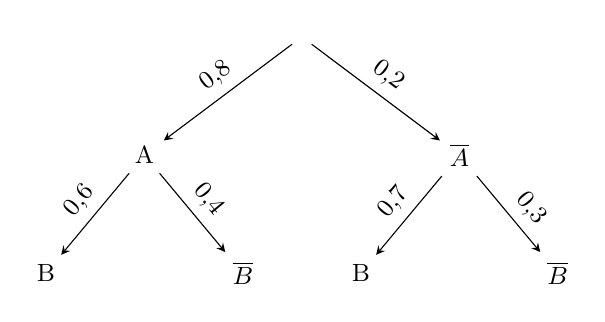
\begin{tikzpicture}[
					level 1/.style={sibling distance=4cm, level distance=1.5cm},
					level 2/.style={sibling distance=2.5cm, level distance=1.5cm},
					level 3/.style={sibling distance=1.5cm, level distance=1.5cm},
					every node/.style={font=\small},
					edge from parent/.style={draw, -{stealth}},
					every path/.style={font=\tiny},
					probability/.style={midway, above, sloped}]
					\node {}
					child { node {A}
						child { node {B}
							edge from parent node [pos=0.5, above,sloped] {0{,}6}
						}
						child { node {$\overline{B}$}
							edge from parent node [pos=0.5, above,sloped] {0{,}4}
						}
						edge from parent node [pos=0.5,above,sloped] {0{,}8}
					}
					child { node {$\overline{A}$}
						child { node {B}
							edge from parent node [pos=0.5, above, sloped] {0{,}7}
						}
						child { node {$\overline{B}$}
							edge from parent node [pos=0.6, above, sloped] {0{,}3}
						}
						edge from parent node [pos=0.5, above,sloped] {0{,}2}
					};
				\end{tikzpicture}
			\end{center}
			\itemch Xác suất để một học sinh đó đỗ đại học với điều kiện học sinh đó chọn tổ hợp $D01$ là
			$$\mathrm{P}\left(B\mid A\right)=0{,}6.$$
			\itemch Xác suất để một học sinh đó đỗ đại học đồng thời học sinh đó chọn tổ hợp $D01$ là
			$$\mathrm{P}\left(AB\right)=\mathrm{P}\left(A\right)\cdot\mathrm{P}\left(B\mid A\right)=0{,}8\cdot0{,}6=0{,}48=\dfrac{12}{25}.$$
			\itemch Xác suất để học sinh đó chọn tổ hợp $D01$ biết rằng học sinh này đã đỗ đại học
			$$\mathrm{P}\left(A\mid B\right)=\dfrac{\mathrm{P}\left(AB\right)}{\mathrm{P}\left(B\right)}=\dfrac{0{,}48}{0{,}8\cdot0{,}6+0{,}2\cdot0{,}7}=\dfrac{24}{31}.$$
		\end{itemchoice}
	}
\end{ex}
%%%=============================%%%
\Closesolutionfile{ans}
\ind{PHẦN III.} \inden{Câu trả lời ngắn.}\\
\setcounter{ex}{0}
\Opensolutionfile{ans}[ans/2T6-Bai1-TLN]
%%%=============EX_1=============%%%	
\begin{ex}[Trích đề thi thử số 2- Bộ 30 đề thi thử MAPSTUDY - Năm học: 2024 - 2025]%[2D6V1-4]
	\immini{Cho lưới ô vuông gồm $6 \times 8$ hình vuông đơn vị. Gọi $M$ là điểm nằm ở góc trái dưới và $N$ là điểm nằm ở góc phải trên của lưới ô vuông. Ngoài ra ta lấy hai điểm $A$, $B$ như hình vẽ.
		Để đi từ điểm $M$ đến điểm $N$ trên lưới ô vuông, một con kiến di chuyển ngẫu nhiên sang phải hoặc lên trên theo các đoạn thẳng là các cạnh của các hình vuông đơn vị.
		Xét hai biến cố:
		\begin{itemize}
			\item $A$: \lq\lq Con kiến đi từ $M$ qua $A$ và đến $N$\rq\rq.
			\item $B$: \lq\lq Con kiến đi từ $M$ qua $B$ và đến $N$\rq\rq.
	\end{itemize}}
	{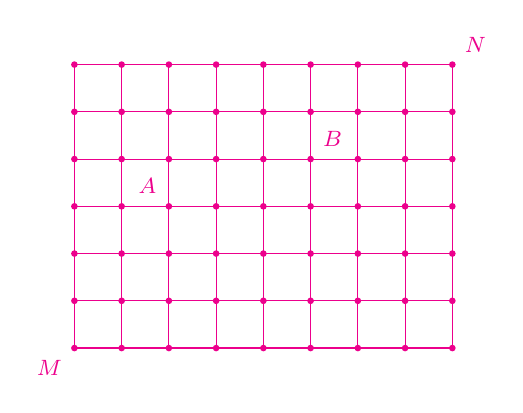
\begin{tikzpicture}[scale=.8, font=\footnotesize, line join=round, line cap=round, >=stealth]
			\def\unit{0.75cm}
			\colorlet{mycolor}{magenta}
			\def\maxx{8}
			\def\maxy{6}
			\draw[step=\unit, thin, mycolor] (0,0) grid (\maxx*\unit, \maxy*\unit);
			\foreach \x in {0,...,\maxx} {
				\foreach \y in {0,...,\maxy} {
					\fill[mycolor] (\x*\unit, \y*\unit) circle (1.5pt);
				}
			}
			\coordinate (M) at (0, 0);
			\coordinate (N) at (\maxx*\unit, \maxy*\unit);
			\coordinate (A) at (2*\unit, 3*\unit);
			\coordinate (B) at (5*\unit, 4*\unit);
			\node[mycolor, below left=1pt] at (M) {$M$};
			\node[mycolor, above right=1pt] at (N) {$N$};
			\node[mycolor, above left=1pt] at (A) {$A$};
			\node[mycolor, above right=1pt] at (B) {$B$};
	\end{tikzpicture}}
	Gọi $a=\mathrm{P}(A\mid B)$ và $b=\mathrm{P}(B\mid A)$. Tính $a+b$ (kết quả làm tròn đến hàng phần mười).
	\par
	\shortans[oly]{0{,}6}
	\loigiai{
		Để đi từ $M$ tới $A$ có $2$ lần sang phải và $3$ lần lên trên nên có $\mathrm{C}_5^2$ (cách).\\
		Để đi từ $A$ tới $N$ có $6$ lần sang phải và $3$ lần lên trên nên có 
		$\mathrm{C}_9^6$ (cách).\\
		Vậy để đi từ $M$ qua $A$ tới $N$ có $n(A)= \mathrm{C}_5^2\cdot \mathrm{C}_9^6=840$ (cách).\\
		Tương tự đi từ $M$ qua $B$ tới $N$ có $n(B)= \mathrm{C}_{10}^6\cdot \mathrm{C}_4^2=1260$ (cách).\\
		Đi từ $M$ tới $A$, tới $B$ rồi tới $N$ là $n(A \cap B)=\mathrm{C}_5^2 \cdot \mathrm{C}_5^4 \cdot \mathrm{C}_4^2=300$ (cách).\\
		Ta có $$a=\mathrm{P}(A \mid B)=\dfrac{\mathrm{P}(A B)}{\mathrm{P}(B)}=\dfrac{n(A \cap B)}{n(B)}=\dfrac{300}{1260}\, \text{và} \,b=P(B \mid A)=\dfrac{\mathrm{P}(B A)}{\mathrm{P}(A)}=\dfrac{n(A \cap B)}{n(A)}=\dfrac{300}{840}.$$
		Vậy $a+b=\dfrac{25}{42}\approx0{,}6$.
	}
\end{ex}
%%%=============================%%%

%%%=============EX_2=============%%%
\begin{ex}[Trích đề thi thử số 1 - Bộ đề thi thử của thầy Phan Nhật Linh - Năm học: 2024-2025]%[2D6V1-2]%[Dự án đề cương 3 khối NH24-25-Dot 1-Khắc Thiên]
	Có hai chiếc hộp, hộp $I$ có $6$ quả bóng màu đỏ và $4$ quả bóng màu vàng, hộp $II$ có $7$ quả bóng màu đỏ và $3$ quả bóng màu vàng, các quả bóng có cùng kích thước và khối lượng. Lấy ngẫu nhiên một quả bóng từ hộp $I$ bỏ vào hộp $II$. Sau đó, lấy ra ngẫu nhiên một quả bóng từ hộp $II$. Tính xác suất để quả bóng được lấy ra từ hộp $II$ là quả bóng được chuyển từ hộp $I$ sang, biết rằng quả bóng đó có màu đỏ (làm tròn kết quả đến hàng phần trăm).
	\par
	\shortans[oly]{0{,}08}
	\loigiai{
		Gọi $A$ là biến cố \lq\lq lấy ra từ hộp $II$ là quả bóng được chuyển từ hộp $I$ sang\rq\rq;\\
		$B$ là biến cố \lq\lq lấy ra từ hộp $II$ là quả bóng màu đỏ\rq\rq.\\
		Ta cần tính $\mathrm{P}\left(A\mid B\right)=\dfrac{\mathrm{P}\left(A\cap B\right)}{\mathrm{P}\left(B\right)}=\dfrac{n\left(A\cap B\right)}{n\left(B\right)}$.\\
		Đếm $n\left(B\right)$ bằng cách chia hai trường hợp như sau
		\begin{itemize}
			\item \textbf{Trường hợp 1:} Lấy một quả đỏ từ hộp $I$ sang hộp $II$ rồi lấy một quả đỏ một quả đỏ từ hộp $II$ thì có tất cả $6\cdot 8=48$ cách.
			\item \textbf{Trường hợp 2:} Lấy một quả vàng từ hộp $I$ sang hộp $II$ rồi lấy một quả đỏ một quả đỏ từ hộp $II$ thì có tất cả $4\cdot 7=28$ cách.
		\end{itemize}
		Suy ra $n\left(B\right)=48+28=76$.\\
		Đếm $n\left(A\cap B\right)$:\\ $A\cap B$ là biến cố lấy một quả đỏ từ hộp $I$ sang hộp $II$ rồi lấy quả đỏ đó từ hộp $II$ ra ngoài nên khi đó $n\left(A\cap B\right)=6\cdot 1=6$.\\
		Do đó $\mathrm{P}\left(A\mid B\right)=\dfrac{6}{76}\approx 0{,}08$.
	}
\end{ex}
%%%=============================%%%

%%%=============EX_3=============%%%
\begin{ex}[Trích đề thi thử số 17 - Bộ 30 đề thi thử MAPSTUDY - Năm học: 2024 - 2025]%[2D6V1-2]
	Có $6$ viên bi đôi một khác nhau, gồm $2$ viên bi màu xanh, $2$ viên bi màu đỏ và $2$ viên bi màu vàng. Xếp ngẫu nhiên $6$ viên bi đó thành một hàng ngang. Tính xác suất để hai viên bi màu vàng đứng cạnh nhau, biết hai viên bi màu xanh không đứng cạnh nhau? (kết quả làm tròn đến hàng phần chục).
	\begin{center}
		
\begin{tikzpicture}[line join = round, line cap = round,>=stealth,font=\footnotesize,scale=1.3]
			\draw[ball color=blue] (0,0) circle (10pt) ;
			\draw[ball color=blue] (1,0) circle (10pt);
			\draw[ball color=red] (2,0) circle (10pt);
			\draw[ball color=red] (3,0) circle (10pt);
			\draw[ball color=yellow] (4,0) circle (10pt);
			\draw[ball color=yellow] (5,0) circle (10pt);
		\end{tikzpicture}
	\end{center}
	\par
	\shortans[oly]{0{,}3}
	\loigiai{
		Gọi $A$ là biến cố \lq\lq Hai bi vàng cạnh nhau\rq\rq\ . \\
		Gọi $B$ là biến cố \lq\lq Hai bi xanh không cạnh nhau\rq\rq\ . \\
		Ta cần tính $\mathrm{P}(A\mid B)=\dfrac{n(AB)}{n(B)}$.\\
		Trước hết ta tính $n(B)$.\\
		Xếp $4$ viên bi không phải màu xanh có $4!$ cách.\\
		$4$ viên bi đó tạo thành $5$ khoảng trống, ta xếp $2$ bi xanh vào $5$ khoảng trống đó, có $\mathrm{A}_5^2$ cách.\\
		Vậy theo quy tắc nhân có $4!\cdot \mathrm{A}_5^2$ cách.\\
		Tiếp theo ta tính $n(AB)$, coi $2$ bi vàng là $1$ vị trí.\\
		Xếp cụm $2$ bi vàng và $2$ bi đỏ, có $3!$ cách.\\
		Tạo thành $4$ khoảng trống, ta xếp $2$ bi xanh vào $4$ khoảng trống đó, có $\mathrm{A}_4^2$ cách.\\
		Vậy $n(AB)=3!\cdot 2!\cdot\mathrm{A}_4^2$.\\
		Vậy $\mathrm{P}(A\mid B)=\dfrac{n(AB)}{n(B)}=\dfrac{3}{10}=0{,}3$.
	}
\end{ex}
%%%=============================%%%

%%%=============EX_4=============%%%
\begin{ex}[Trích đề thi thử thực chiến 13 - Bộ đề thi thử thầy Đỗ Văn Đức - Năm học: 2024 - 2025]%[2D6C1-2]
	Một hộp có $12$ viên bi, gồm $6$ bi xanh và $6$ bi đỏ. Lấy ra ngẫu nhiên $8$ viên bi từ hộp. Tính xác suất để trong $8$ viên bi lấy ra có ít nhất $4$ viên bi xanh, biết trong $8$ bi lấy ra có ít nhất $2$ viên bi xanh (kết quả làm tròn đến hàng phần trăm).
	\par
	\shortans[oly]{0{,}73}
	\loigiai{
		Gọi $A$ là sự kiện \lq\lq trong $8$ viên bi lấy ra có ít nhất $4$ viên bi xanh\rq\rq.\\
		Gọi $B$ là sự kiện \lq\lq trong $8$ viên bi lấy ra có ít nhất $2$ viên bi xanh\rq\rq.\\
		Ta cần tính xác suất có điều kiện $\mathrm{P}(A\mid B) = \dfrac{\mathrm{P}(A \cap B)}{\mathrm{P}(B)}$.\\
		Nếu sự kiện $A$ xảy ra (có ít nhất $4$ bi xanh), thì chắc chắn sự kiện $B$ cũng xảy ra (vì nếu có ít nhất $4$ bi xanh thì cũng có ít nhất $2$ bi xanh).\\
		Do đó $A \cap B = A$.\\
		Vậy $\mathrm{P}(A\mid B) = \dfrac{\mathrm{P}(A)}{\mathrm{P}(B)}$.\\
		Tổng số cách lấy ngẫu nhiên $8$ viên bi từ $12$ viên bi là
		$n(\Omega)=\mathrm{C}_{12}^{8}=495$.\\
		Xét sự kiện $B\colon$ \lq\lq trong $8$ bi lấy ra có ít nhất $2$ viên bi xanh\rq\rq.\\
		Khi lấy $8$ viên bi từ $6$ bi xanh và $6$ bi đỏ, số bi xanh tối thiểu có thể lấy được là $8 - 6= 2$.\\
		Số bi xanh tối đa có thể lấy được là $6$.\\
		Như vậy, mọi cách lấy $8$ viên bi từ hộp này đều sẽ có ít nhất 2 viên bi xanh.\\
		Do đó, $B$ là biến cố chắc chắn.\\
		Số phần tử của $B$ là $n(B) = n(\Omega) = 495$.\\
		Xác suất của $B$ là $\mathrm{P}(B) = \dfrac{n(B)}{n(\Omega)} = \dfrac{495}{495} = 1$.\\
		Xét sự kiện $A\colon$ \lq\lq trong $8$ viên bi lấy ra có ít nhất $4$ viên bi xanh\rq\rq. Các trường hợp xảy ra:
		\begin{itemize}
			\item Lấy được $4$ bi xanh và $4$ bi đỏ $\mathrm{C}_{6}^{4}\cdot\mathrm{C}_{6}^{4}= 225$ (cách).
			\item Lấy được $5$ bi xanh và $3$ bi đỏ $\mathrm{C}_{6}^{5}\cdot\mathrm{C}_{6}^{3}= 120$ (cách).
			\item Lấy được $6$ bi xanh và $2$ bi đỏ $\mathrm{C}_{6}^{6}\cdot\mathrm{C}_{6}^{2}= 15$ (cách).
		\end{itemize}
		Số phần tử của $A$ là $n(A) = 225 + 120 + 15 = 360$.\\
		Xác suất của $A$ là $\mathrm{P}(A) = \dfrac{n(A)}{n(\Omega)} = \dfrac{360}{495}$.\\
		Vậy xác suất cần tìm là
		$\mathrm{P}(A\mid B) = \dfrac{\mathrm{P}(A)}{\mathrm{P}(B)} = \dfrac{360}{495} =\dfrac{8}{11} \approx 0{,}73.$
	}
\end{ex}
%%%=============================%%%

%%%=============EX_5=============%%%
\begin{ex}[Trích đề thi thử số 25 - Bộ 30 đề thi thử MAPSTUDY - Năm học: 2024-2025]%[2D6C1-2]%[Dự án đề cương 3 khối NH24-25-Dot 1-Khắc Thiên]
	Ba người cùng ngắm bắn súng vào mục tiêu thì thấy chỉ có $2$ người bắn trúng đích. Biết xác suất bắn trúng đích của mỗi người lần lượt là $0{,}6$; $0{,}8$ và $0{,}9$. Tìm xác suất để người thứ nhất bắn trúng đích (kết quả làm tròn đến hàng phần trăm).
	\par
	\shortans[oly]{0{,}35}
	\loigiai{
		Xét biến cố $A\colon$ \lq\lq$3$ người cùng ngắm bắn, có $2$ người bắn trúng đích\rq\rq.\\
		Xét biến cố $B\colon$ \lq\lq Người thứ nhất bắn trúng đích\rq\rq.\\
		Khi đó, $\mathrm{P}(B)=0{,}6$.\\	Ta cần tính $\mathrm{P}(B\mid A)=\dfrac{\mathrm{P}(BA)}{\mathrm{P}(A)}$.\\
		Giả sử $A_{i}$ là biến cố \lq\lq Người thứ $i$ bắn trúng đích\rq\rq\,với $i=1,2,3$.\\
		Khi đó, ta có
		\allowdisplaybreaks
		\begin{eqnarray*}
			\mathrm{P}\left(A\right)&=&\mathrm{P}\left( \overline{A_{1}}A_{2}A_{3}\cup A_{1}\overline{A_{2}}A_{3} \cup A_{1}A_{2}\overline{A_{3}}\right)\\
			&=&\mathrm{P}\left(\overline{A_{1}}\right)\cdot \mathrm{P}\left(A_{2}\right)\cdot \mathrm{P}\left(A_{3}\right)+\mathrm{P}\left(A_{1}\right)\cdot \mathrm{P}\left(\overline{A_{2}}\right)\cdot \mathrm{P}\left(A_{3}\right) +\mathrm{P}\left(A_{1}\right)\cdot \mathrm{P}\left(A_{2}\right)\cdot \mathrm{P}\left(\overline{A_{3}}\right)\\
			&=&(1-0{,}6)\cdot0{,}8\cdot0{,}9+0{,}6\cdot(1-0{,}8)\cdot0{,}9+0{,}6\cdot0{,}8\cdot(1-0{,}9)\\
			&=&0{,}444.\\
			\mathrm{P}\left(BA\right)&=&\mathrm{P}\left(A_{1}\overline{A_{2}}A_{3} \cup A_{1}A_{2}\overline{A_{3}}\right)=0{,}6\cdot(1-0{,}8)\cdot0{,}9+0{,}6\cdot0{,}8\cdot(1-0{,}9)\\
			&=&0{,}156.\\
			\Rightarrow \mathrm{P}\left(B\mid A\right)&=&\dfrac{\mathrm{P}\left(BA\right)}{\mathrm{P}\left(A\right)}=\dfrac{0{,}156}{0{,}444}=\dfrac{13}{37}\approx 0{,}35.
		\end{eqnarray*}
	}
\end{ex}
%%%=============================%%%
\Closesolutionfile{ans}

\ind{PHẦN IV.} \inden{Tự luận.}\\
\setcounter{ex}{0}
%%%=============EX_1=============%%%
\begin{ex}[SGK Toán 12 - Chân trời sáng tạo]%[2D5N1-2]%[Dự án đề cương 3 khối NH24-25-Dot 1-Khắc Thiên]
	Một thư viện có $35\%$ tổng số sách là sách khoa học, $14\%$ tổng số sách là sách khoa học tự nhiên. Chọn ngẫu nhiên một quyển sách của thư viện. Tính xác suất để quyển sách được chọn là sách khoa học tự nhiên, biết rằng đó là quyển sách về khoa học.
	\loigiai{
		Gọi $A$ là biến cố \lq\lq Sách được chọn là sách khoa học tự nhiên\rq\rq.\\
		Gọi $B$ là biến cố \lq\lq Sách được chọn là sách khoa học\rq\rq.\\
		Do có $35\%$ tổng số sách là sách khoa học nên $\mathrm{P}\left(B\right)=0{,}35$.\\
		Do có $14\%$ tổng số sách là sách khoa học tự nhiên nên $\mathrm{P}\left(AB\right)=0{,}14$.\\
		Vậy $\mathrm{P}\left(A\mid B\right)=\dfrac{\mathrm{P}\left(AB\right)}{\mathrm{P}\left(B\right)}=\dfrac{0{,}14}{0{,}35}=0{,}4$.
	}
\end{ex}
%%%=============================%%%

%%%=============EX_2=============%%%
\begin{ex}[SGK Toán 12 - Cùng khám phá]%[2D5N1-2]%[Dự án đề cương 3 khối NH24-25-Dot 1-Khắc Thiên]
	Một hộp có $5$ viên bi cùng kích thước và khối lượng, trong đó có $3$ viên bi màu đỏ và $2$ viên bi màu xanh. Lấy ngẫu nhiên lần lượt $2$ viên bi và không hoàn lại. Tính xác suất để lấy được viên bi thứ hai có màu xanh, biết rằng viên bi thứ nhất có màu đỏ.
	\loigiai{
		Gọi
		\begin{itemize}
			\item $A$ là biến cố \lq\lq Lấy được viên bi thứ hai có màu xanh\rq\rq;
			\item $B$ là biến cố \lq\lq Lấy được viên bi thứ nhất có màu đỏ\rq\rq.
		\end{itemize}
		Khi đó xác suất để lấy được viên bi thứ hai có màu xanh, biết rằng viên bi thứ nhất có màu đỏ chính là xác suất của $A$ với điều kiện $B$.\\
		Vì một viên bi đỏ đã được lấy ra ở lần thứ nhất nên trong hộp còn lại $4$ viên bi, trong đó có $2$ viên bi xanh.\\
		Từ đó ta có $\mathrm{P}(A \mid B)=\dfrac{2}{4}=0{,}5$.\\
		Vậy xác suất để lấy được viên bi thứ hai có màu xanh, biết rằng viên bi thứ nhất có màu đỏ là $0{,}5$.
	}
\end{ex}
%%%=============================%%%

%%%=============EX_3=============%%%
\begin{ex}[Trích đề thi HKII - Trường THPT Lê Quý Đôn - Quảng Ngãi - Năm học: 2024-2025]%[2D6N1-2]%[Dự án đề cương 3 khối NH24-25-Dot 1-Khắc Thiên]
	Cho $\mathrm{P}\left(A\right)=0{,}3$; $\mathrm{P}\left(B\right)=0{,}5$; $\mathrm{P}\left(B\mid A\right)=0{,}7$. Tính
	$\mathrm{P}\left(A\mid B\right)$.
	\loigiai{
		Ta có $\mathrm{P}\left(A\mid B\right)=\dfrac{\mathrm{P}\left(A\right)\cdot \mathrm{P}\left(B\mid A\right)}{\mathrm{P}\left(B\right)}=0{,}42$.}
\end{ex}
%%%=============================%%%

%%%=============EX_4=============%%%
\begin{ex}[SGK Toán 12 - Cánh diều]%[2D6N1-2]%[Dự án đề cương 3 khối NH24-25-Dot 1-Khắc Thiên]
	Cho hai biến cố $A$, $B$ có $\mathrm{P}\left(A\right)=0{,}6$; $\mathrm{P}\left(B\right)=0{,}8$; $\mathrm{P}\left(A\cap B\right)=0{,}4$. Tính các xác suất sau:
	\begin{listEX}[2]
		\item $\mathrm{P}\left(B\mid A\right)$; $\mathrm{P}\left(\overline{B}\mid A\right)$.
		\item $\mathrm{P}\left(A \cap \overline{B}\right)$.
	\end{listEX}
	\loigiai{
		\begin{enumerate}
			\item $\mathrm{P}\left(B\mid A\right)=\dfrac{\mathrm{P}\left(A \cap B\right)}{\mathrm{P}\left(A\right)}=\dfrac{0{,}4}{0{,}6}=\dfrac{2}{3}
			\Rightarrow \mathrm{P}\left(\overline{B}\mid A\right)=1-\mathrm{P}\left(B\mid A\right)= 1-\dfrac{2}{3}=\dfrac{1}{3}$.
			\item Ta có
			$\mathrm{P}\left(A \cap \overline{B}\right)= \mathrm{P}\left(\overline{B}\mid A\right)\cdot \mathrm{P} \left(A\right)=\dfrac{1}{3}\cdot 0{,}6=0{,}2$.
	\end{enumerate}}
\end{ex}
%%%=============================%%%

%%%=============EX_5=============%%%
\begin{ex}[SGK Toán 12 - Cánh diều]%[2D6H1-2]%[Dự án đề cương 3 khối NH24-25-Dot 1-Khắc Thiên]
	Cho hai con xúc xắc cân đối và đồng chất. Gieo lần lượt từng xúc xắc trong hai xúc xắc đó. Tính xác suất để tổng số chấm xuất hiện trên hai xúc xắc bằng $6$, biết rằng xúc xắc thứ nhất xuất hiện mặt $4$ chấm.
	\loigiai{
		Gọi $A$ là biến cố \lq\lq xúc xắc thứ nhất xuất hiện mặt $4$ chấm\rq\rq ~và $B$ là biến cố \lq\lq tổng số chấm xuất hiện trên hai xúc xắc bằng $6$\rq\rq.\\
		Xác suất của $A$ là $\mathrm{P}\left(A\right)$ là xác suất để xúc xắc thứ nhất xuất hiện mặt $4$ chấm. Vì xúc xắc cân đối và đồng chất, nên $\mathrm{P}\left(A\right)=\dfrac{1}{6}$.\\
		Xác suất của $B$ khi biết $A$ đã xảy ra là $\mathrm{P}\left(B \mid A\right)$.\\ Trong trường hợp này, để tổng số chấm là $6$, xúc xắc thứ hai phải xuất hiện mặt $2$ chấm.\\ Do đó, $\mathrm{P}\left(B \mid A\right)=\dfrac{1}{6}$.\\
		Vậy theo quy tắc xác suất điều kiện, ta có
		$$\mathrm{P}\left(B \mid A\right)=\dfrac{\mathrm{P}\left(A \cap B\right)}{\mathrm{P}\left(A\right)} \Rightarrow \mathrm{P}\left(A \cap B\right)=\mathrm{P}\left(B \mid A\right)\cdot \mathrm{P}\left(A\right)=\dfrac{1}{6}\cdot \dfrac{1}{6}=\dfrac{1}{36}.$$
	}
\end{ex}
%%%=============================%%%

%%%=============EX_6=============%%%
\begin{ex}[SGK Toán 12 - Cánh diều]%[2D6H1-2]%[Dự án đề cương 3 khối NH24-25-Dot 1-Khắc Thiên]
	Một lô sản phẩm có $20$ sản phẩm, trong đó có $5$ sản phẩm chất lượng thấp. Lấy liên tiếp $2$ sản phẩm trong lô sản phẩm trên, trong đó sản phẩm lấy ra ở lần thứ nhất không được bỏ lại vào lô sản phẩm. Tính xác suất để cả hai sản phẩm được lấy ra đều có chất lượng thấp.
	\loigiai{
		Gọi $A$ là biến cố \lq\lq sản phẩm thứ nhất có chất lượng thấp\rq\rq~và $B$ là biến cố \lq\lq sản phẩm thứ hai có chất lượng thấp\rq\rq.\\
		Xác suất của $A$ là xác suất để lấy ra một sản phẩm chất lượng thấp trong lần đầu tiên
		$$\mathrm{P}\left(A\right)=\dfrac{n\left(A\right)}{n\left(\Omega\right)}=\dfrac{5}{20}=\dfrac{1}{4}.$$
		Sau khi lấy một sản phẩm chất lượng thấp, số sản phẩm chất lượng thấp giảm còn $4$ trong tổng số $19$ sản phẩm.\\
		Xác suất của $B$ khi đã xảy ra $A$ là xác suất để lấy ra một sản phẩm chất lượng thấp trong lần thứ hai
		$\mathrm{P}\left(B \mid A\right)=\dfrac{4}{19}$.\\
		Áp dụng quy tắc nhân xác suất
		$\mathrm{P}\left(A \cap B\right)=\mathrm{P}\left(A\right)\cdot \mathrm{P}\left(B \mid A\right)=\dfrac{1}{4}\cdot\dfrac{4}{19}=\dfrac{1}{19}$.\\
		Vậy xác suất để cả hai sản phẩm được lấy ra đều có chất lượng thấp là $\dfrac{1}{19}$.
	}
\end{ex}
%%%=============================%%%

%%%=============EX_7=============%%%
\begin{ex}[SGK Toán 12 - Chân trời sáng tạo]%[2D5H1-2]%[Dự án đề cương 3 khối NH24-25-Dot 1-Khắc Thiên]
	Cho hai biến cố $A$ và $B$ có $\mathrm{P}\left( A\right)=0{,}4$; $\mathrm{P}\left(B\right)=0{,}8$ và $\mathrm{P}\left(A\mid B\right)=0{,}5$. Tính $\mathrm{P}\left(A\overline{B}\right)$ và $\mathrm{P}\left(A\mid B\right)$.
	\loigiai{
		Ta có $\mathrm{P}\left(A\overline{B}\right)=\mathrm{P}\left(A\mid\overline{B}\right)\cdot \mathrm{P}\left(\overline{B}\right)=0{,}5\cdot 0{,}2=0{,}1$.\\
		Vì $AB$ và $A\overline{B}$ là hai biến cố xung khắc và $AB\cup A\overline{B}=A$ nên theo tính chất của xác suất, ta có\\ $\mathrm{P}\left(AB\right)=\mathrm{P}\left(A\right)-\mathrm{P}\left(A\overline{B}\right)=0{,}4-0{,}1=0{,}3$.\\
		Khi đó $\mathrm{P}\left(A\mid B\right)=\dfrac{\mathrm{P}\left(AB\right)}{\mathrm{P}\left(B\right)}=\dfrac{0{,}3}{0{,}8}=0{,}375$.
	}
\end{ex}
%%%=============================%%%

%%%=============EX_8=============%%%
\begin{ex}[Trích đề thi HKII - Trường THCS-THPT Trí Đức - TP.HCM - Năm học: 2024-2025]%[2D6V1-3]%[Dự án đề cương 3 khối NH24-25-Dot 1-Khắc Thiên]
	Hiện nay, nước ta đang trong quá trình tinh gọn bộ máy nhà nước và thực hiện nghị quyết không tổ chức công an cấp huyện. Do vậy, trong đợt điều động cán bộ công an từ huyện về công tác tại cơ sở hoặc công tác tại công an tỉnh, phòng tổ chức cán bộ nhận thấy rằng: Có $60\%$ cán bộ có nguyện vọng về công tác tại cơ sở là các xã vùng sâu vùng xa, số còn lại có nguyện vọng về công tác tại công an tỉnh.
	\begin{itemize}
		\item Trong số cán bộ có nguyện vọng về công tác tại cơ sở thì $70\%$ có trình độ đại học và $30\%$ có trình độ trung cấp.
		\item Trong số cán bộ có nguyện vọng về công an tỉnh thì $80\%$ có trình độ đại học và $20\%$ có trình độ trung cấp.
	\end{itemize}
	Tuy nhiên, năng lực công tác cũng là một yếu tố quan trọng. Dựa trên hồ sơ đánh giá năng lực thì
	\begin{itemize}
		\item Trong số cán bộ có nguyện vọng về cơ sở thì tỉ lệ cán bộ được đánh giá có năng lực \lq\lq Tốt\rq\rq\, trở lên với trình độ đại học là $60\%$ và trình độ trung cấp là $30\%$.
		\item Trong số cán bộ có nguyện vọng về công tác tại công an tỉnh thì tỉ lệ được đánh giá là có năng lực \lq\lq Tốt\rq\rq\, trở lên với trình độ đại học là $85\%$ và với trình độ trung cấp là $25\%$.
	\end{itemize}
	Chọn ngẫu nhiên một cán bộ công an. Tính xác suất để cán bộ này vừa có trình độ đại học vừa được đánh giá là có năng lực \lq\lq Tốt\rq\rq\, trở lên và có nguyện vọng về công tác tại cơ sở là các xã vùng sâu, vùng xa.
	\loigiai{
		Gọi $A$ là biến cố \lq\lq Chọn được cán bộ công an có nguyện vọng về cơ sở\rq\rq.\\
		$B$ là biến cố \lq\lq Cán bộ công an được chọn có trình độ đại học\rq\rq. \\
		$C$ là biến cố \lq\lq Cán bộ công an được chọn có năng lực \lq\lq Tốt\rq\rq\ trở lên\rq\rq.\\
		Ta có sơ đồ cây
		\begin{center}
			\begin{tikzpicture}[node distance=2.25cm, every node/.style={fill=white}, align=center]
				%----Thêm \usetikzlibrary{arrows.meta}
				\definecolor{diagram_bg_green}{HTML}{d5e8d4}
				\definecolor{diagram_bg_blue}{HTML}{dae8fc}
				\definecolor{diagram_bg_pink}{HTML}{f8cecc}
				\definecolor{diagram_bd_green}{HTML}{82b366}
				\definecolor{diagram_bd_blue}{HTML}{7494c2}
				\definecolor{diagram_bd_pink}{HTML}{b85450}
				\tikzset{>={Latex[width=2mm,length=2mm]},
					base/.style = {rectangle, rounded corners, draw=black, minimum width=1cm, minimum height=1cm, text centered, drop shadow={shadow xshift=0.6mm, shadow yshift=-0.6mm}},
					Style1/.style = {base, fill=diagram_bg_blue, draw=diagram_bd_blue},
					Style2/.style = {base, fill=diagram_bg_pink, draw=diagram_bd_pink},
					Style3/.style = {base, fill=diagram_bg_green, draw=diagram_bd_green},
					Style4/.style = {base, minimum width=1.5cm, fill=orange!15, draw=orange},
				}
				\node (B0) [Style1, text width=1cm] {Gốc};
				\node (B1) [Style2, right of=B0, xshift=1.5cm, yshift=2cm, text width=1.5cm] {$A$};
				\node (B3) [Style2, right of=B0, xshift=1.5cm, yshift=-2cm, text width=1.5cm] {$\overline{A}$};
				\node (B11) [Style3, right of=B1, xshift=3cm, yshift=1.2cm, text width=1.5cm] {$B$};
				\node (B13) [Style3, right of=B1, xshift=3cm, yshift=-1.2cm, text width=1.5cm] {$\overline{B}$};
				\node (B31) [Style3, right of=B3, xshift=3cm, yshift=1.2cm, text width=1.5cm] {$B$};
				\node (B33) [Style3, right of=B3, xshift=3cm, yshift=-1.2cm, text width=1.5cm] {$\overline{B}$};
				
				\draw[->] (B0) -- (B1.west)node[sloped,above,pos=0.5]{$60$\%};
				\draw[->] (B0) -- (B3.west)node[sloped,below,pos=0.5]{$40$\%};
				\draw[->] (B1) -- (B11.west)node[sloped,above,pos=0.5]{$70$\%};
				\draw[->] (B1) -- (B13.west)node[sloped,below,pos=0.5]{$30$\%};
				\draw[->] (B3) -- (B31.west)node[sloped,above,pos=0.5]{$80$\%};
				\draw[->] (B3) -- (B33.west)node[sloped,below,pos=0.5]{$20$\%};
				
				\node (B111) [Style4, right of=B11, xshift=3.5cm, yshift=1.2cm, text width=1.5cm] {$C$};
				\node (B113) [Style4, right of=B11, xshift=3.5cm, yshift=0cm, text width=1.5cm] {$\overline{C}$};
				\draw[->] (B11) -- (B111.west)node[sloped,above,pos=0.5]{$60$\%};
				\draw[->] (B11) -- (B113.west);
				
				\node (B131) [Style4, right of=B13, xshift=3.5cm, yshift=1.2cm, text width=1.5cm] {$C$};
				\node (B133) [Style4, right of=B13, xshift=3.5cm, yshift=0cm, text width=1.5cm] {$\overline{C}$};
				\draw[->] (B13) -- (B131.west)node[sloped,above,pos=0.5]{$30$\%};
				\draw[->] (B13) -- (B133.west);
				
				\node (B311) [Style4, right of=B31, xshift=3.5cm, yshift=0cm, text width=1.5cm] {$C$};
				\node (B313) [Style4, right of=B31, xshift=3.5cm, yshift=-1.2cm, text width=1.5cm] {$\overline{C}$};
				\draw[->] (B31) -- (B311.west)node[sloped,above,pos=0.5]{$85$\%};
				\draw[->] (B31) -- (B313.west);
				
				\node (B331) [Style4, right of=B33, xshift=3.5cm, yshift=0cm, text width=1.5cm] {$C$};
				\node (B333) [Style4, right of=B33, xshift=3.5cm, yshift=-1.2cm, text width=1.5cm] {$\overline{C}$};
				\draw[->] (B33) -- (B331.west)node[sloped,above,pos=0.5]{$25$\%};
				\draw[->] (B33) -- (B333.west);
			\end{tikzpicture}
		\end{center}
		Vậy xác suất để cán bộ này vừa có trình độ đại học vừa được đánh giá là có năng lực \lq\lq Tốt\rq\rq\, trở lên và vừa có nguyện vọng về công tác tại cơ sở là các xã vùng sâu, vùng xa là
		\begin{center}
			$\mathrm{P}\left(ABC\right)=60\% \cdot 70\% \cdot 60\%=0{,}252$.
		\end{center}
	}
\end{ex}
%%%=============================%%%

%%%=============EX_9=============%%%
\begin{ex}[SGK Toán 12 - Chân trời sáng tạo]%[2D5V1-3]%[Dự án đề cương 3 khối NH24-25-Dot 1-Khắc Thiên]
	Mỗi bạn học sinh trong lớp của Minh lựa chọn một trong hai ngoại ngữ là tiếng Anh hoặc tiếng Nhật. Xác suất chọn tiếng Anh của mỗi bạn học sinh nữ là $0{,}6$ và của mỗi bạn học sinh nam là $0{,}7$. Lớp của Minh có $25$ bạn nữ và $20$ bạn nam. Chọn ra ngẫu nhiên một bạn trong lớp. Sử dụng sơ đồ hình cây, tính xác suất của các biến cố\\
	$A$: \lq\lq Bạn được chọn là nam và học tiếng Nhật\rq\rq.\\
	$B$: \lq\lq Bạn được chọn là nữ và học tiếng Anh\rq\rq.
	\loigiai{
		Số học sinh của lớp là $25+20=45$ (học sinh).\\
		Gọi biến cố $X$: \lq\lq Bạn được chọn là nữ\rq\rq~thì $\overline{X}$ là biến cố \lq\lq Bạn được chọn là nam\rq\rq.\\
		Gọi biến cố $Y$: \lq\lq Bạn được chọn học tiếng Anh\rq\rq~thì $\overline{Y}$ là biến cố \lq\lq Bạn được chọn học tiếng Nhật\lq\lq.\\
		Khi đó ta có biến cố $A=\overline{X}\cdot\overline{Y}$: \lq\lq Bạn được chọn là nam và học tiếng Nhật\rq\rq.\\
		Biến cố $B=XY$: \lq\lq Bạn được chọn là nữ và học tiếng Anh\rq\rq.\\
		Ta có
		$\mathrm{P}\left(X\right)=\dfrac{20}{45}=\dfrac{5}{9}$;
		$\mathrm{P}\left(Y\mid X\right)=0{,}6$; $\mathrm{P}\left(Y \mid \overline{X}\right)=0{,}7$.\\
		Do đó $\mathrm{P}\left(\overline{X}\right)=1-\mathrm{P}\left(X\right)=\dfrac{4}{9}$; $\mathrm{P}\left(\overline{Y}\mid X\right)=1-\mathrm{P}\left(Y\mid X\right)=0{,}4$; $\mathrm{P}\left(\overline{Y} \mid \overline{X}\right)=1-\mathrm{P}\left(Y \mid \overline{X}\right)=0{,}3$.\\
		Ta có sơ đồ hình cây như sau
		\begin{center}
			\begin{tikzpicture}
				\def\gocm{20}
				\def\gocn{10}
				\def\r{4}
				\tikzset{s/.style={outer sep=0.5 mm,draw=magenta,rectangle,minimum width=2.75cm,rounded corners=1mm}}
				\path(0,0)node(O){}++(\gocm:\r)node[s](A1){X}++(\gocn:\r)node[s](A2){$Y$};
				\path(A1)++({-\gocn}:\r)node[s](a2){$\overline{Y}$};
				\path(O)++(-\gocm:\r)node[s](B1){$\overline{X}$}++(\gocn:\r)node[s](B2){$Y$};
				\path(B1)++({-\gocn}:\r)node[s](b2){$\overline{Y}$};
				\foreach \x/\y in {
					O/A1,A1/A2,
					O/B1,B1/B2,
					A1/a2,
					B1/b2}
				\draw[-stealth](\x.east)--(\y.west);
				\path(O)--(A1.west)node[pos=0.5,above]{$\dfrac{5}{9}$}(O)--(B1.west)node[pos=0.5,below]{$\dfrac{4}{9}$}(B1.east)--(B2.west)node[pos=0.5,above,sloped]{$0{,}7$}(A1.east)--(A2.west)node[pos=0.5,above,sloped]{$0{,}6$}
				(A1.east)--(a2.west)node[pos=0.5,below,sloped]{$0{,}4$}
				(B1.east)--(b2.west)node[pos=0.5,below,sloped]{$0{,}3$};
			\end{tikzpicture}
		\end{center}
		Vì $A=\overline{X}\cdot\overline{Y}$ nên $\mathrm{P}\left(\overline{X}\cdot\overline{Y}\right)=\dfrac{4}{9}\cdot 0{,}3=\dfrac{2}{15}$.\\
		Vì $B=XY$ nên $\mathrm{P}\left(XY\right)=\dfrac{5}{9}\cdot 0{,}6=\dfrac{1}{3}$.\\
	}
\end{ex}
%%%=============================%%%

%%%=============EX_10=============%%%
\begin{ex}[SGK Toán 12 - Cánh diều]%[2D6V1-2]%[Dự án đề cương 3 khối NH24-25-Dot 1-Khắc Thiên]
	Một doanh nghiệp trước khi xuất khẩu áo sơ mi phải qua hai lần kiểm tra chất lượng sản phẩm, nếu cả hai lần đều đạt thì chiếc áo đó mới đủ tiêu chuẩn xuất khẩu. Biết rằng bình quân $98\%$ sản phẩm làm ra qua được lần kiểm tra thứ nhất và $95\%$ sản phẩm qua được lần kiểm tra thứ nhất sẽ tiếp tục qua được lần kiểm tra thứ hai. Tính xác suất để một chiếc áo sơ mi đủ tiêu chuẩn xuất khẩu.
	\loigiai{
		$A$ là biến cố \lq\lq sản phẩm qua được lần kiểm tra thứ nhất\rq\rq.\\
		$B$ là biến cố \lq\lq sản phẩm qua được lần kiểm tra thứ hai\rq\rq.\\
		Bài toán yêu cầu tính xác suất của biến cố $A\cap B$, tức là sản phẩm vừa qua được lần kiểm tra thứ nhất, và sau đó qua được lần kiểm tra thứ hai.\\
		Xác suất của $A$ là $\mathrm{P}\left(A\right)=0{,}98$.\\
		Xác suất của $B$ khi đã qua được $A$ là $\mathrm{P}\left(B \mid A\right)=0{,}95$.\\
		Áp dụng công thức xác suất có điều kiện, ta có
		\begin{eqnarray*}
			\mathrm{P}\left(A \cap B\right)=\mathrm{P}\left(A\right)\cdot \mathrm{P}\left(B \mid A\right)=0{,}98\cdot 0{,}95=0{,}931.
		\end{eqnarray*}
		Vậy xác suất để một chiếc áo sơ mi đủ tiêu chuẩn xuất khẩu là $93{,}1\%$.
	}
\end{ex}
%%%=============================%%% 